\section{同変Schubert計算における組合せ論}
\subsection{Schubert puzzleによる方法}

\begin{defin}
  図\ref{puzzle piece}の$8$種類のラベル付きの図形をpuzzle pieceと呼ぶ.

  \begin{figure}[htbp]
    \centering
    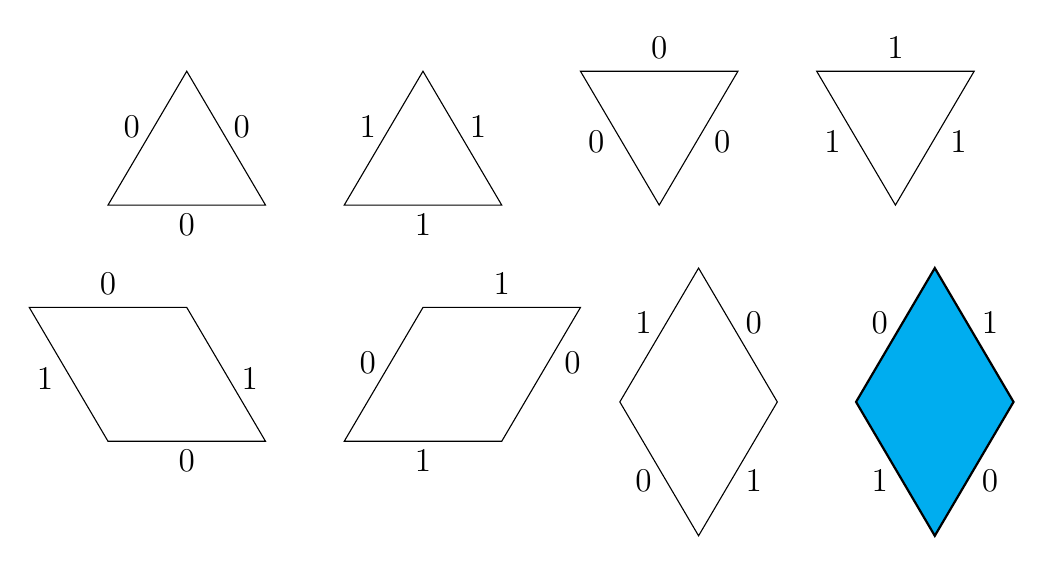
\begin{tikzpicture}
      \coordinate (A) at (0,0);
      \coordinate (B) at (2,0);
      \coordinate (C) at (1,1.7);

      \draw (A)--(B)--(C)--cycle;
      \node[font=\large] at ($(A)+(1,-0.25)$) {$0$};
      \node[font=\large] at ($(A)+(0.3,1)$) {$0$};
      \node[font=\large] at ($(A)+(1.7,1)$) {$0$};

      \coordinate(P) at (3,0);
      \draw ($(A)+(P)$)--($(B)+(P)$)--($(C)+(P)$)--cycle;
      \node[font=\large] at ($(P)+(1,-0.25)$) {$1$};
      \node[font=\large] at ($(P)+(0.3,1)$) {$1$};
      \node[font=\large] at ($(P)+(1.7,1)$) {$1$};

      \coordinate (Q) at (6,0);
      \draw ($(A)+(Q)+(0,1.7)$)--($(B)+(Q)+(0,1.7)$)--($(C)+(Q)-(0,1.7)$)--cycle;
      \node[font=\large] at ($(Q)+(0.2,0.8)$) {$0$};
      \node[font=\large] at ($(Q)+(1.8,0.8)$) {$0$};
      \node[font=\large] at ($(Q)+(1,2)$) {$0$};

      \coordinate (R) at (9,0);
      \draw ($(A)+(R)+(0,1.7)$)--($(B)+(R)+(0,1.7)$)--($(C)+(R)-(0,1.7)$)--cycle;
      \node[font=\large] at ($(R)+(0.2,0.8)$) {$1$};
      \node[font=\large] at ($(R)+(1.8,0.8)$) {$1$};
      \node[font=\large] at ($(R)+(1,2)$) {$1$};

      \draw ($(A)-(0,3)$)--($(B)-(0,3)$)--($(C)-(0,3)$)--($(C)-(2,3)$)--cycle; 
      \node[font=\large] at ($(A)+(1,-3.25)$) {$0$};
      \node[font=\large] at ($(A)+(1.8,-2.2)$) {$1$};
      \node[font=\large] at ($(A)+(-0.8,-2.2)$) {$1$};
      \node[font=\large] at ($(A)+(0,-1)$) {$0$};

      \draw ($(A)-(-3,3)$)--($(B)-(-3,3)$)--($(C)-(-5,3)$)--($(C)-(-3,3)$)--cycle;
      \node[font=\large] at ($(P)+(1,-3.25)$) {$1$};
      \node[font=\large] at ($(P)+(2.9,-2)$) {$0$};
      \node[font=\large] at ($(P)+(0.3,-2)$) {$0$};
      \node[font=\large] at ($(P)+(2,-1)$) {$1$}; 

      \draw ($(A)+(6.5,-2.5)$)--($(C)+(6.5,-2.5)$)--($(B)+(6.5,-2.5)$)--($(C)+(6.5,-5.9)$)--cycle;
      \node[font=\large] at ($(Q)+(0.8,-1.5)$) {$1$};
      \node[font=\large] at ($(Q)+(2.2,-1.5)$) {$0$};
      \node[font=\large] at ($(Q)+(2.2,-3.5)$) {$1$};
      \node[font=\large] at ($(Q)+(0.8,-3.5)$) {$0$};

      \fill[cyan] ($(A)+(9.5,-2.5)$)--($(C)+(9.5,-2.5)$)--($(B)+(9.5,-2.5)$)--($(C)+(9.5,-5.9)$)--cycle;
      \draw[thick] ($(A)+(9.5,-2.5)$)--($(C)+(9.5,-2.5)$)--($(B)+(9.5,-2.5)$)--($(C)+(9.5,-5.9)$)--cycle;
      \node[font=\large] at ($(R)+(0.8,-1.5)$) {$0$};
      \node[font=\large] at ($(R)+(2.2,-1.5)$) {$1$};
      \node[font=\large] at ($(R)+(2.2,-3.5)$) {$0$};
      \node[font=\large] at ($(R)+(0.8,-3.5)$) {$1$};
    \end{tikzpicture}
    \caption{$8$種類のpuzzle piece.}\label{puzzle piece}
  \end{figure}
  ただし,puzzle pieceのうち三角形のものは$1$辺の長さが$1$の正三角形であり,平行四辺形のものは$1$辺の長さが$1$で鋭角は$60$度であるとする.またpuzzle pieceのうち
    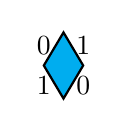
\begin{tikzpicture}[baseline=-1pt]
      \fill[cyan] (0,0)--(0.25,0.42)--(0.5,0)--(0.25,-0.42)--cycle;
      \draw[thick] (0,0)--(0.25,0.42)--(0.5,0)--(0.25,-0.42)--cycle;
      \node at (0,0.25) {$0$};
      \node at (0.5,0.25) {$1$};
      \node at (0,-0.25) {$1$};
      \node at (0.5,-0.25) {$0$};
    \end{tikzpicture}
  をequivariant pieceという.
\end{defin}

\begin{defin}
  いくつかのpuzzle pieceを(同一種のpieceは何個用いてもよい)同じラベルを持つ辺に沿って貼り合わせ,一つの大きな正三角形を作ったものをpuzzleと呼ぶ.puzzle $P$を上向きの正三角形となるように見たとき,$P$の左上の辺上に存在するラベルたちを下から上に読んで得られる文字列を$\lambda$,$P$の右上の辺上に存在するラベルたちを上から下に読んで得られる文字列を$\mu$,下の辺上に存在するラベルたちを左から右に読んで得られる文字列を$\nu$とする.このとき$\partial P = \Delta^{\nu}_{\lambda\mu}$と表す.
\end{defin}

\begin{eg}
  $\partial P=\Delta^{1010}_{0110,1001}$をみたすpuzzleは図\ref{0110,1001,1010}のpuzzleのみである.

  \begin{figure}[htbp]
    \centering
    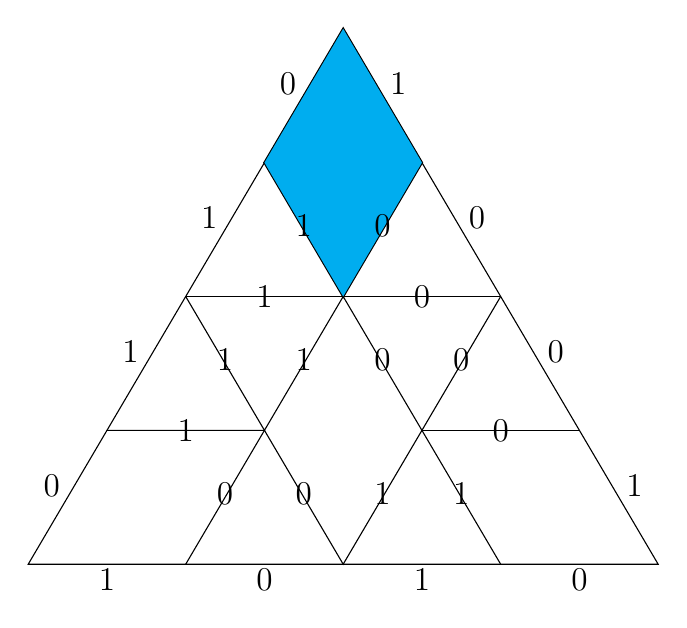
\begin{tikzpicture}
      \draw (0,0)--(8,0)--(4,6.8)--cycle;
      \draw (2,0)--(3,1.7)--(1,1.7);
      \draw (3,1.7)--(4,0)--(5,1.7)--(6,0);
      \draw (5,1.7)--(7,1.7);

      \draw (2,3.4)--(3,1.7)--(4,3.4)--(5,1.7)--(6,3.4);
      \draw (2,3.4)--(6,3.4);

      \draw[thick] (3,5.1)--(4,3.4)--(5,5.1)--(4,6.8)--cycle;
      \fill[cyan] (3,5.1)--(4,3.4)--(5,5.1)--(4,6.8)--cycle;

      \node[font=\large] at (1,-0.2) {$1$};
      \node[font=\large] at (3,-0.2) {$0$};
      \node[font=\large] at (5,-0.2) {$1$};
      \node[font=\large] at (7,-0.2) {$0$};

      \node[font=\large] at (2,1.7) {$1$};
      \node[font=\large] at (6,1.7) {$0$};

      \node[font=\large] at (3,3.4) {$1$};
      \node[font=\large] at (5,3.4) {$0$};


      \coordinate (A) at (0.3, 1);
      \coordinate (P) at (1,1.7);
      \node[font=\large] at (A) {$0$};
      \node[font=\large] at ($(A)+(P)$) {$1$};
      \node[font=\large] at ($(A)+2*(P)$) {$1$};
      \node[font=\large] at ($(A)+3*(P)$) {$0$};

      \coordinate (B) at (7.7, 1);
      \coordinate (Q) at (-1,1.7);
      \node[font=\large] at (B) {$1$};
      \node[font=\large] at ($(B) + (Q)$) {$0$};
      \node[font=\large] at ($(B) + 2*(Q)$) {$0$};
      \node[font=\large] at ($(B) + 3*(Q)$) {$1$};

      \node[font=\large] at (2.5,0.9) {$0$};
      \node[font=\large] at (3.5,0.9) {$0$};
      \node[font=\large] at (4.5,0.9) {$1$};
      \node[font=\large] at (5.5,0.9) {$1$};
      
      \node[font=\large] at (2.5,2.6) {$1$};
      \node[font=\large] at (3.5,2.6) {$1$};
      \node[font=\large] at (4.5,2.6) {$0$};
      \node[font=\large] at (5.5,2.6) {$0$};

      \node[font=\large] at (3.5,4.3) {$1$};
      \node[font=\large] at (4.5,4.3) {$0$};
    \end{tikzpicture}
    \caption{$\partial P=\Delta^{1010}_{0110,1001}$をみたすただ一つのpuzzle}\label{0110,1001,1010}
  \end{figure}
\end{eg}

\begin{defin}
  $1$辺の長さが$n$のpuzzle $P$に含まれるequivariant piece $p$に対して,そのウェイト$\text{wt}(p)\in\integer[y_1,\cdots,y_n]$を次のように定義する.$p$の重心から,$P$の下辺に向かって$P$の左上の辺と平行な直線を引き,その交点が位置するpuzzle pieceの辺が左から数えて$i$番目にあるとする.次に$p$の重心から,$P$の下辺に向かって$P$の右上の辺と平行な直線を引き,その交点が位置するpuzzle pieceの辺が左から数えて$j$番目にあるとする.このとき
  \[
  \text{wt}(p)=y_j-y_i
  \]
  とする(図\ref{puzzle weight}).
\end{defin}

\begin{figure}[htbp]
  \centering
  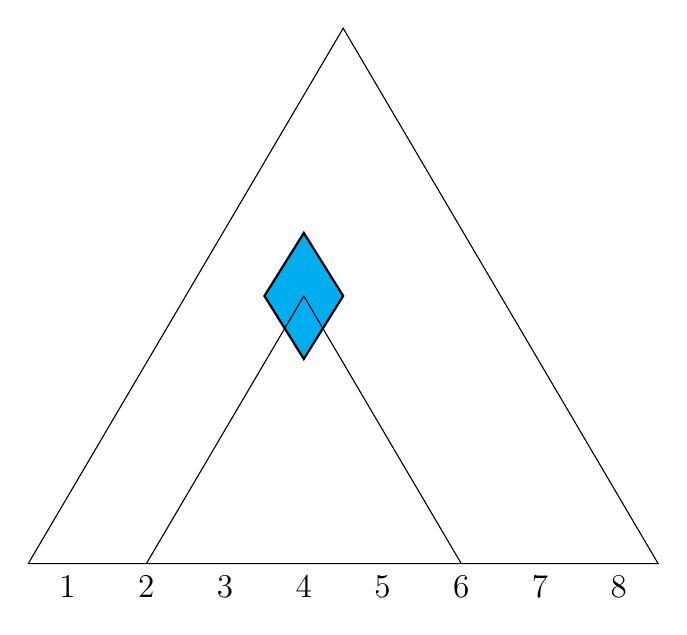
\begin{tikzpicture}
    \draw (0,0)--(8,0)--(4,6.8)--cycle;
    \fill[cyan] (3,3.4)--(3.5,2.6)--(4,3.4)--(3.5,4.2)--cycle;
    \draw[thick] (3,3.4)--(3.5,2.6)--(4,3.4)--(3.5,4.2)--cycle;
    
    \draw (3.5,3.4)--(1.5,0);
    \draw (3.5,3.4)--(5.5,0);


    \node[font=\large] at (0.5,-0.3) {$1$};
    \node[font=\large] at (1.5,-0.3) {$2$};
    \node[font=\large] at (2.5,-0.3) {$3$};
    \node[font=\large] at (3.5,-0.3) {$4$};
    \node[font=\large] at (4.5,-0.3) {$5$};
    \node[font=\large] at (5.5,-0.3) {$6$};
    \node[font=\large] at (6.5,-0.3) {$7$};
    \node[font=\large] at (7.5,-0.3) {$8$};
  \end{tikzpicture}
  \caption{equivariant pieceのウェイトの定義.図のequivariant pieceのウェイトは$\text{wt}(p)=y_6-y_2$である.}\label{puzzle weight}
\end{figure}


\begin{defin}
  puzzle $P$に対してそのウェイト$\text{wt}(P)$を
  \[
  \text{wt}(P):=\prod_{p:\text{ equivariant piece}}\text{wt}(p)
  \]
  とする.
\end{defin}

式(\ref{LRcoeff})の係数$C^\nu_{\lambda\mu}$に関して次が成り立つ.

\begin{theo}(Knutson-Tao \cite{knutson tao})
  \[
  C^\nu_{\lambda\mu}=\prod_{\substack{P:\text{ puzzle} \\ \partial P = \Delta^\nu_{\lambda\mu}}}\text{wt}(P)
  \]
  が成り立つ.
\end{theo}



\subsection{edge labeled tableauxによる方法}

\begin{defin}
  $n$の分割$\lambda=(\lambda_1\geq\cdots\geq\lambda_k>0)$に対して,$1$行目に$\lambda_1$個の箱を, $2$行目に$\lambda_2$個の箱を,順に$k$行目まで左寄せで書いた図をYoung図形という.以降分割とYoung図形を同一視して同じ記号で表す.$\lambda$の各箱に,各行について左から右に単調増大, 各列について上から下に単調増大となるように相異なる数字を$1$回ずつ書き入れたものをstandard tableauxという.
\end{defin}

\begin{eg}
\[
\ytableausetup{nobaseline}
\ydiagram{5, 3, 3, 1}
\quad\begin{ytableau}
    1&3&5&6&12\\
    2&4&8\\
    7&9&10\\
    11
\end{ytableau}
\]
\begin{figure}[htbp]
  \centering
  \caption{$\lambda=(5,3,3,1)$のYoung図形とその上のstandard tableauxの例}
\end{figure}
\end{eg}


\begin{defin}\label{label condition}
  分割$\lambda, \mu$に対して,$\lambda\leq\mu\Leftrightarrow \lambda_i\leq\mu_i\:(\forall i)$によって順序を定める.$\lambda<\mu$を満たすYoung図形に対して,$\mu$のYoung図形から$\lambda$に相当する部分を取り除いた図形を歪Young図形といい$\mu/\lambda$で表す.整数$n>0$を固定する. 歪Young図形の各箱に$1$から$n$までの数字を書き入れ,水平方向の各辺に$\{1,\cdots,n\}$の部分集合(空でもよい)を書き入れたものを, equivariant fillingという.equivariant fillingのうち,次の条件を満たすものをequivariant standard tableauxという.
  \begin{itemize}
    \item $1$から$n$までの各数字が,いずれかの箱のラベルに現れるか,またはいずれかの辺のラベルの要素になっている.また$1$から$n$までの各数字がちょうど1回現れる.
    \item 各箱のラベルについて,左隣の箱のラベルよりも大きい.
    \item 各箱のラベルについて,上辺のラベルが空でないなら,その最大値よりも大きい.空であるならば,すぐ上の箱のラベルより大きい.
    \item 各辺のラベルについて,そのすべての数字がすぐ上の箱に書かれたラベルよりも大きい.
  \end{itemize}
  形が$\mu/\lambda$で$1$から$n$までの数字が書かれたequivariant standard tableauxの全体の集合を$\text{EqSYT}(\mu/\lambda, n)$とする.
\end{defin}

\begin{eg}\label{example of EqSYT}
  図\ref{eg of 4331/221}は$(4,3,3,1)/(2,2,1)$上のequivariant standard tableauxの例と$(4,4,2)/(3,3,1)$上のequivariant standard tableauxの例である.
  \begin{figure}
    \centering
    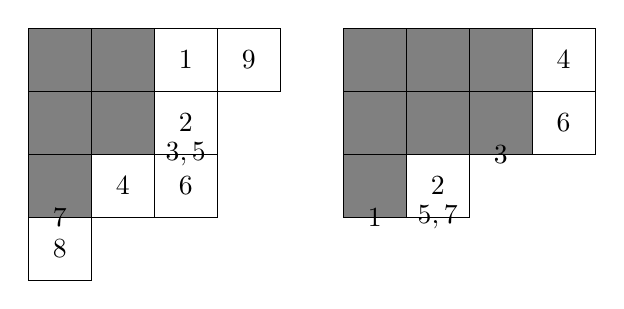
\begin{tikzpicture}
      \begin{scope}
        \fill[gray] (0,0)--(1.6,0)--(1.6,-1.6)--(0.8,-1.6)--(0.8,-2.4)--(0,-2.4)--cycle;
        \draw (0,0)--(0,-3.2)--(0.8,-3.2)--(0.8,-2.4)--(2.4,-2.4)--(2.4,-0.8)--(3.2,-0.8)--(3.2,0)--cycle;
        \draw (0,-0.8)--(2.4,-0.8);
        \draw (0,-1.6)--(2.4,-1.6);
        \draw (0,-2.4)--(0.8,-2.4);
        \draw (0.8,0)--(0.8,-2.4);
        \draw (1.6,0)--(1.6,-2.4);
        \draw (2.4,0)--(2.4,-0.8);
  
        \node at (2,-0.4) {$1$};
        \node at (2.8,-0.4) {$9$};
        \node at (2,-1.2) {$2$};
        \node at (1.2,-2) {$4$};
        \node at (2,-2) {$6$};
        \node at (0.4,-2.8) {$8$};
  
        \node at (0.4,-2.4) {$7$};
        \node at (2,-1.6) {$3,5$};
      \end{scope}
      \begin{scope}[xshift=4cm]
        \fill[gray] (0,0)--(2.4,0)--(2.4,-1.6)--(0.8,-1.6)--(0.8,-2.4)--(0,-2.4)--cycle;
        \draw (0,0)--(3.2,0)--(3.2,-1.6)--(1.6,-1.6)--(1.6,-2.4)--(0,-2.4)--cycle;
        \draw (0.8,0)-- +(0,-2.4);
        \draw (1.6,0)-- +(0,-1.6);
        \draw (2.4,0)-- +(0,-1.6);
        \draw (0,-0.8)-- +(3.2,0);
        \draw (0,-1.6)-- +(1.6,0);
  
        \node at (2.8,-0.4) {$4$};
        \node at (2.8,-1.2) {$6$};
        \node at (1.2,-2) {$2$};
        \node at (0.4,-2.4) {$1$};
        \node at (1.2,-2.4) {$5,7$};
        \node at (2,-1.6) {$3$};
      \end{scope}
    \end{tikzpicture}
    \caption{$(4,3,3,1)/(2,2,1)$上のequivariant standard tableauxの例(左)と$(4,4,2)/(3,3,1)$上のequivariant standard tableauxの例(右)}\label{eg of 4331/221}
  \end{figure}
\end{eg}

\begin{defin}
  $\lambda$の箱$x$が$T\in\text{EqSYT}(\mu/\lambda, n)$の内隅であるとは,$x$のすぐ右とすぐ下の箱が$\lambda$の箱でないことをいう.また$\mu/\lambda$の箱$x$が外隅であるとは,$x$のすぐ右とすぐ下の箱が存在しないことをいう.$T$の内隅$x$に対して,次の操作を考える:
  \begin{enumerate}
    \item $x$の下辺のラベル$l$が空でないなら,$l$の最小値を$x$のラベルに移す
    \item $x$の下辺のラベルが空であるとし,$x$のすぐ右の箱を$y$,すぐ下の箱を$z$とする.$y$と$z$のうち,ラベルの小さい方の箱を$x$と交換する(このとき辺のラベルは交換しない).
  \end{enumerate}
  (i)の操作が行われる,もしくは$x$が外隅になるまで(i),(ii)を繰り返してできるtableauxを$T$の$x$によるequivariant jeu de taquin といい,$\text{EqJdt}_x(T)$と書く.
\end{defin}

\begin{defin}
  $\lambda$の箱を各列に沿って下から上に,右から左に数えて$x_1,\cdots,x_m$とする.$T\in\text{EqSYT}(\mu/\lambda, n)$に対して,$T$のequivariant rectificationを$x_1$から順に$x_m$までequivariant jeu de taquinを行って得られるtableauxとする.すなわち
  \[
  \text{EqRect}(T):=\text{EqJdt}_{x_m}(\text{EqJdt}_{x_{m-1}}(\cdots(\text{EqJdt}_{x_1}(T))\cdots))
  \]
  をTのequivariant rectificationという.
\end{defin}

\begin{eg}\label{fst calculation}
  図\ref{eg of 4331/221}左のtableauxのequivariant rectificationを図示する(図\ref{rect of 4331/221}).
  \begin{figure}[H]
    \centering
    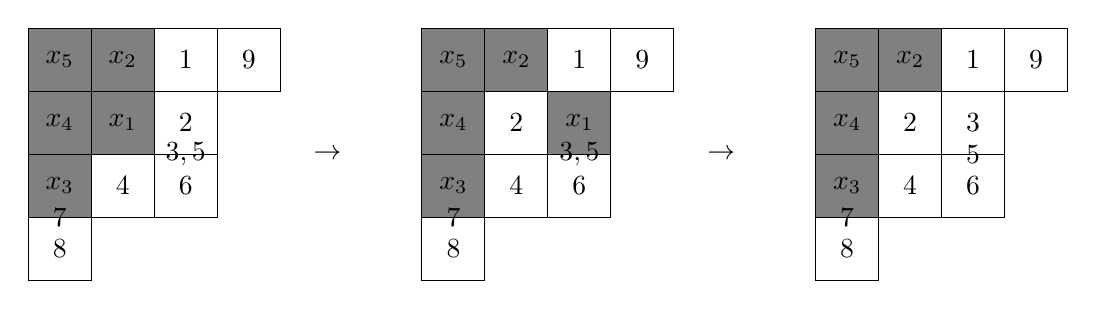
\begin{tikzpicture}
      \begin{scope}
        \fill[gray] (0,0)--(1.6,0)--(1.6,-1.6)--(0.8,-1.6)--(0.8,-2.4)--(0,-2.4)--cycle;
        \draw (0,0)--(0,-3.2)--(0.8,-3.2)--(0.8,-2.4)--(2.4,-2.4)--(2.4,-0.8)--(3.2,-0.8)--(3.2,0)--cycle;
        \draw (0,-0.8)--(2.4,-0.8);
        \draw (0,-1.6)--(2.4,-1.6);
        \draw (0,-2.4)--(0.8,-2.4);
        \draw (0.8,0)--(0.8,-2.4);
        \draw (1.6,0)--(1.6,-2.4);
        \draw (2.4,0)--(2.4,-0.8);
  
        \node at (2,-0.4) {$1$};
        \node at (2.8,-0.4) {$9$};
        \node at (2,-1.2) {$2$};
        \node at (1.2,-2) {$4$};
        \node at (2,-2) {$6$};
        \node at (0.4,-2.8) {$8$};
  
        \node at (0.4,-2.4) {$7$};
        \node at (2,-1.6) {$3,5$};

        \node at (1.2,-1.2) {$x_1$};
        \node at (1.2,-0.4) {$x_2$};
        \node at (0.4,-2) {$x_3$};
        \node at (0.4,-1.2) {$x_4$};
        \node at (0.4,-0.4) {$x_5$};
        \node at (3.8,-1.6) {$\rightarrow$};
      \end{scope}
      \begin{scope}[xshift=5cm]
        \fill[gray] (0,0)--(1.6,0)--(1.6,-0.8)--(0.8,-0.8)--(0.8,-2.4)--(0,-2.4)--cycle;
        \fill[gray] (1.6,-0.8) rectangle (2.4,-1.6);
        \draw (0,0)--(0,-3.2)--(0.8,-3.2)--(0.8,-2.4)--(2.4,-2.4)--(2.4,-0.8)--(3.2,-0.8)--(3.2,0)--cycle;
        \draw (0,-0.8)--(2.4,-0.8);
        \draw (0,-1.6)--(2.4,-1.6);
        \draw (0,-2.4)--(0.8,-2.4);
        \draw (0.8,0)--(0.8,-2.4);
        \draw (1.6,0)--(1.6,-2.4);
        \draw (2.4,0)--(2.4,-0.8);
  
        \node at (2,-0.4) {$1$};
        \node at (2.8,-0.4) {$9$};
        \node at (2,-1.2) {$x_1$};
        \node at (1.2,-2) {$4$};
        \node at (2,-2) {$6$};
        \node at (0.4,-2.8) {$8$};
  
        \node at (0.4,-2.4) {$7$};
        \node at (2,-1.6) {$3,5$};
        \node at (1.2,-1.2) {$2$};

        \node at (1.2,-0.4) {$x_2$};
        \node at (0.4,-2) {$x_3$};
        \node at (0.4,-1.2) {$x_4$};
        \node at (0.4,-0.4) {$x_5$};

        \node at (3.8,-1.6) {$\rightarrow$};
      \end{scope}
      \begin{scope}[xshift=10cm]
        \fill[gray] (0,0)--(1.6,0)--(1.6,-0.8)--(0.8,-0.8)--(0.8,-2.4)--(0,-2.4)--cycle;
        \draw (0,0)--(0,-3.2)--(0.8,-3.2)--(0.8,-2.4)--(2.4,-2.4)--(2.4,-0.8)--(3.2,-0.8)--(3.2,0)--cycle;
        \draw (0,-0.8)--(2.4,-0.8);
        \draw (0,-1.6)--(2.4,-1.6);
        \draw (0,-2.4)--(0.8,-2.4);
        \draw (0.8,0)--(0.8,-2.4);
        \draw (1.6,0)--(1.6,-2.4);
        \draw (2.4,0)--(2.4,-0.8);
  
        \node at (2,-0.4) {$1$};
        \node at (2.8,-0.4) {$9$};
        \node at (2,-1.2) {$3$};
        \node at (1.2,-2) {$4$};
        \node at (2,-2) {$6$};
        \node at (0.4,-2.8) {$8$};
  
        \node at (0.4,-2.4) {$7$};
        \node at (2,-1.6) {$5$};
        \node at (1.2,-1.2) {$2$};
        
        \node at (1.2,-0.4) {$x_2$};
        \node at (0.4,-2) {$x_3$};
        \node at (0.4,-1.2) {$x_4$};
        \node at (0.4,-0.4) {$x_5$};
      \end{scope}
    \end{tikzpicture}

    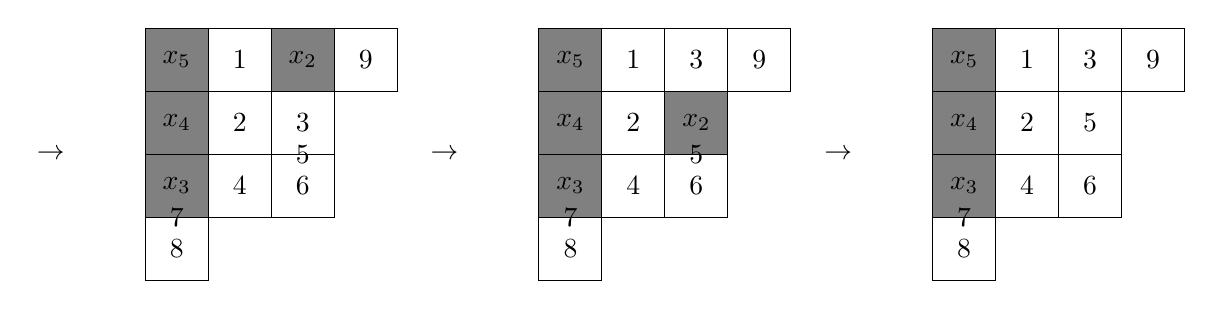
\begin{tikzpicture}
      \begin{scope}
        \fill[gray] (0,0)--(0.8,0)--(0.8,-2.4)--(0,-2.4)--cycle;
        \fill[gray] (1.6,0) rectangle (2.4,-0.8);
        \draw (0,0)--(0,-3.2)--(0.8,-3.2)--(0.8,-2.4)--(2.4,-2.4)--(2.4,-0.8)--(3.2,-0.8)--(3.2,0)--cycle;
        \draw (0,-0.8)--(2.4,-0.8);
        \draw (0,-1.6)--(2.4,-1.6);
        \draw (0,-2.4)--(0.8,-2.4);
        \draw (0.8,0)--(0.8,-2.4);
        \draw (1.6,0)--(1.6,-2.4);
        \draw (2.4,0)--(2.4,-0.8);
  
        \node at (2,-0.4) {$x_2$};
        \node at (2.8,-0.4) {$9$};
        \node at (2,-1.2) {$3$};
        \node at (1.2,-2) {$4$};
        \node at (2,-2) {$6$};
        \node at (0.4,-2.8) {$8$};
  
        \node at (0.4,-2.4) {$7$};
        \node at (2,-1.6) {$5$};
        \node at (1.2,-1.2) {$2$};
        
        \node at (1.2,-0.4) {$1$};
        \node at (0.4,-2) {$x_3$};
        \node at (0.4,-1.2) {$x_4$};
        \node at (0.4,-0.4) {$x_5$};
        \node at (-1.2,-1.6) {$\rightarrow $};
        \node at (3.8,-1.6) {$\rightarrow $};
      \end{scope}
      \begin{scope}[xshift=5cm]
        \fill[gray] (0,0)--(0.8,0)--(0.8,-2.4)--(0,-2.4)--cycle;
        \fill[gray] (1.6,-0.8) rectangle (2.4,-1.6);
        \draw (0,0)--(0,-3.2)--(0.8,-3.2)--(0.8,-2.4)--(2.4,-2.4)--(2.4,-0.8)--(3.2,-0.8)--(3.2,0)--cycle;
        \draw (0,-0.8)--(2.4,-0.8);
        \draw (0,-1.6)--(2.4,-1.6);
        \draw (0,-2.4)--(0.8,-2.4);
        \draw (0.8,0)--(0.8,-2.4);
        \draw (1.6,0)--(1.6,-2.4);
        \draw (2.4,0)--(2.4,-0.8);
  
        \node at (2,-0.4) {$3$};
        \node at (2.8,-0.4) {$9$};
        \node at (2,-1.2) {$x_2$};
        \node at (1.2,-2) {$4$};
        \node at (2,-2) {$6$};
        \node at (0.4,-2.8) {$8$};
  
        \node at (0.4,-2.4) {$7$};
        \node at (2,-1.6) {$5$};
        \node at (1.2,-1.2) {$2$};
        
        \node at (1.2,-0.4) {$1$};
        \node at (0.4,-2) {$x_3$};
        \node at (0.4,-1.2) {$x_4$};
        \node at (0.4,-0.4) {$x_5$};
        \node at (3.8,-1.6) {$\rightarrow $};
      \end{scope}
      \begin{scope}[xshift=10cm]
        \fill[gray] (0,0)--(0.8,0)--(0.8,-2.4)--(0,-2.4)--cycle;
        \draw (0,0)--(0,-3.2)--(0.8,-3.2)--(0.8,-2.4)--(2.4,-2.4)--(2.4,-0.8)--(3.2,-0.8)--(3.2,0)--cycle;
        \draw (0,-0.8)--(2.4,-0.8);
        \draw (0,-1.6)--(2.4,-1.6);
        \draw (0,-2.4)--(0.8,-2.4);
        \draw (0.8,0)--(0.8,-2.4);
        \draw (1.6,0)--(1.6,-2.4);
        \draw (2.4,0)--(2.4,-0.8);
  
        \node at (2,-0.4) {$3$};
        \node at (2.8,-0.4) {$9$};
        \node at (2,-1.2) {$5$};
        \node at (1.2,-2) {$4$};
        \node at (2,-2) {$6$};
        \node at (0.4,-2.8) {$8$};
  
        \node at (0.4,-2.4) {$7$};
        \node at (1.2,-1.2) {$2$};
        
        \node at (1.2,-0.4) {$1$};
        \node at (0.4,-2) {$x_3$};
        \node at (0.4,-1.2) {$x_4$};
        \node at (0.4,-0.4) {$x_5$};
      \end{scope}
    \end{tikzpicture}

    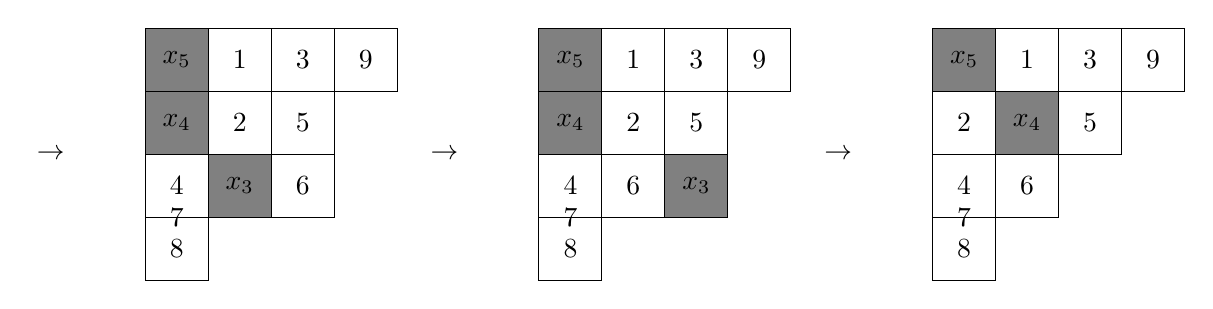
\begin{tikzpicture}
      \begin{scope}
        \fill[gray] (0,0) rectangle (0.8,-1.6);
        \fill[gray] (0.8,-1.6) rectangle (1.6,-2.4);
        \draw (0,0)--(0,-3.2)--(0.8,-3.2)--(0.8,-2.4)--(2.4,-2.4)--(2.4,-0.8)--(3.2,-0.8)--(3.2,0)--cycle;
        \draw (0,-0.8)--(2.4,-0.8);
        \draw (0,-1.6)--(2.4,-1.6);
        \draw (0,-2.4)--(0.8,-2.4);
        \draw (0.8,0)--(0.8,-2.4);
        \draw (1.6,0)--(1.6,-2.4);
        \draw (2.4,0)--(2.4,-0.8);
  
        \node at (2,-0.4) {$3$};
        \node at (2.8,-0.4) {$9$};
        \node at (2,-1.2) {$5$};
        \node at (1.2,-2) {$x_3$};
        \node at (2,-2) {$6$};
        \node at (0.4,-2.8) {$8$};
  
        \node at (1.2,-1.2) {$2$};
        
        \node at (1.2,-0.4) {$1$};
        \node at (0.4,-2) {$4$};
        \node at (0.4,-2.4) {$7$};
        \node at (0.4,-1.2) {$x_4$};
        \node at (0.4,-0.4) {$x_5$};
        \node at (-1.2,-1.6) {$\rightarrow $};
        \node at (3.8,-1.6) {$\rightarrow $};
      \end{scope}
      \begin{scope}[xshift=5cm]
        \fill[gray] (0,0) rectangle (0.8,-1.6);
        \fill[gray] (1.6,-1.6) rectangle (2.4,-2.4);
        \draw (0,0)--(0,-3.2)--(0.8,-3.2)--(0.8,-2.4)--(2.4,-2.4)--(2.4,-0.8)--(3.2,-0.8)--(3.2,0)--cycle;
        \draw (0,-0.8)--(2.4,-0.8);
        \draw (0,-1.6)--(2.4,-1.6);
        \draw (0,-2.4)--(0.8,-2.4);
        \draw (0.8,0)--(0.8,-2.4);
        \draw (1.6,0)--(1.6,-2.4);
        \draw (2.4,0)--(2.4,-0.8);
  
        \node at (2,-0.4) {$3$};
        \node at (2.8,-0.4) {$9$};
        \node at (2,-1.2) {$5$};
        \node at (1.2,-2) {$6$};
        \node at (2,-2) {$x_3$};
        \node at (0.4,-2.8) {$8$};
  
        \node at (1.2,-1.2) {$2$};
        
        \node at (1.2,-0.4) {$1$};
        \node at (0.4,-2) {$4$};
        \node at (0.4,-2.4) {$7$};
        \node at (0.4,-1.2) {$x_4$};
        \node at (0.4,-0.4) {$x_5$};
        \node at (3.8,-1.6) {$\rightarrow $};
      \end{scope}
      \begin{scope}[xshift=10cm]
        \fill[gray] (0,0) rectangle (0.8,-0.8);
        \fill[gray] (0.8,-0.8) rectangle (1.6,-1.6);
        \draw (0,0)--(0,-3.2)--(0.8,-3.2)--(0.8,-2.4)--(1.6,-2.4)--(1.6,-1.6)--(2.4,-1.6)--(2.4,-0.8)--(3.2,-0.8)--(3.2,0)--cycle;
        \draw (0,-0.8)--(2.4,-0.8);
        \draw (0,-1.6)--(2.4,-1.6);
        \draw (0,-2.4)--(0.8,-2.4);
        \draw (0.8,0)--(0.8,-2.4);
        \draw (1.6,0)--(1.6,-2.4);
        \draw (2.4,0)--(2.4,-0.8);
  
        \node at (2,-0.4) {$3$};
        \node at (2.8,-0.4) {$9$};
        \node at (2,-1.2) {$5$};
        \node at (1.2,-2) {$6$};
        \node at (0.4,-2.8) {$8$};
  
        \node at (1.2,-1.2) {$x_4$};
        
        \node at (1.2,-0.4) {$1$};
        \node at (0.4,-2) {$4$};
        \node at (0.4,-2.4) {$7$};
        \node at (0.4,-1.2) {$2$};
        \node at (0.4,-0.4) {$x_5$};
      \end{scope}
    \end{tikzpicture}

    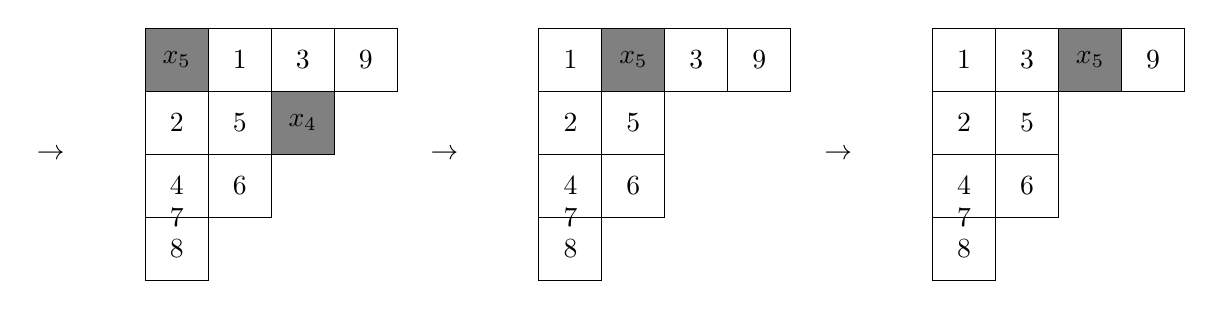
\begin{tikzpicture}
      \begin{scope}
        \fill[gray] (0,0) rectangle (0.8,-0.8);
        \fill[gray] (1.6,-0.8) rectangle (2.4,-1.6);
        \draw (0,0)--(0,-3.2)--(0.8,-3.2)--(0.8,-2.4)--(1.6,-2.4)--(1.6,-1.6)--(2.4,-1.6)--(2.4,-0.8)--(3.2,-0.8)--(3.2,0)--cycle;
        \draw (0,-0.8)--(2.4,-0.8);
        \draw (0,-1.6)--(2.4,-1.6);
        \draw (0,-2.4)--(0.8,-2.4);
        \draw (0.8,0)--(0.8,-2.4);
        \draw (1.6,0)--(1.6,-2.4);
        \draw (2.4,0)--(2.4,-0.8);
  
        \node at (2,-0.4) {$3$};
        \node at (2.8,-0.4) {$9$};
        \node at (2,-1.2) {$x_4$};
        \node at (1.2,-2) {$6$};
        \node at (0.4,-2.8) {$8$};
  
        \node at (1.2,-1.2) {$5$};
        
        \node at (1.2,-0.4) {$1$};
        \node at (0.4,-2) {$4$};
        \node at (0.4,-2.4) {$7$};
        \node at (0.4,-1.2) {$2$};
        \node at (0.4,-0.4) {$x_5$};

        \node at (-1.2,-1.6) {$\rightarrow $};
        \node at (3.8,-1.6) {$\rightarrow $};
      \end{scope}
      \begin{scope}[xshift=5cm]
        \fill[gray] (0.8,0) rectangle (1.6,-0.8);
        \draw (0,0)--(0,-3.2)--(0.8,-3.2)--(0.8,-2.4)--(1.6,-2.4)--(1.6,-0.8)--(3.2,-0.8)--(3.2,0)--cycle;
        \draw (0,-0.8)--(2.4,-0.8);
        \draw (0,-1.6)--(1.6,-1.6);
        \draw (0,-2.4)--(0.8,-2.4);
        \draw (0.8,0)--(0.8,-2.4);
        \draw (1.6,0)--(1.6,-2.4);
        \draw (2.4,0)--(2.4,-0.8);
  
        \node at (2,-0.4) {$3$};
        \node at (2.8,-0.4) {$9$};
        \node at (1.2,-2) {$6$};
        \node at (0.4,-2.8) {$8$};
  
        \node at (1.2,-1.2) {$5$};
        
        \node at (1.2,-0.4) {$x_5$};
        \node at (0.4,-2) {$4$};
        \node at (0.4,-2.4) {$7$};
        \node at (0.4,-1.2) {$2$};
        \node at (0.4,-0.4) {$1$};

        \node at (3.8,-1.6) {$\rightarrow $};
      \end{scope}
      \begin{scope}[xshift=10cm]
        \fill[gray] (1.6,0) rectangle (2.4,-0.8);
        \draw (0,0)--(0,-3.2)--(0.8,-3.2)--(0.8,-2.4)--(1.6,-2.4)--(1.6,-0.8)--(3.2,-0.8)--(3.2,0)--cycle;
        \draw (0,-0.8)--(2.4,-0.8);
        \draw (0,-1.6)--(1.6,-1.6);
        \draw (0,-2.4)--(0.8,-2.4);
        \draw (0.8,0)--(0.8,-2.4);
        \draw (1.6,0)--(1.6,-2.4);
        \draw (2.4,0)--(2.4,-0.8);
  
        \node at (2,-0.4) {$x_5$};
        \node at (2.8,-0.4) {$9$};
        \node at (1.2,-2) {$6$};
        \node at (0.4,-2.8) {$8$};
  
        \node at (1.2,-1.2) {$5$};
        
        \node at (1.2,-0.4) {$3$};
        \node at (0.4,-2) {$4$};
        \node at (0.4,-2.4) {$7$};
        \node at (0.4,-1.2) {$2$};
        \node at (0.4,-0.4) {$1$};
      \end{scope}
    \end{tikzpicture}

    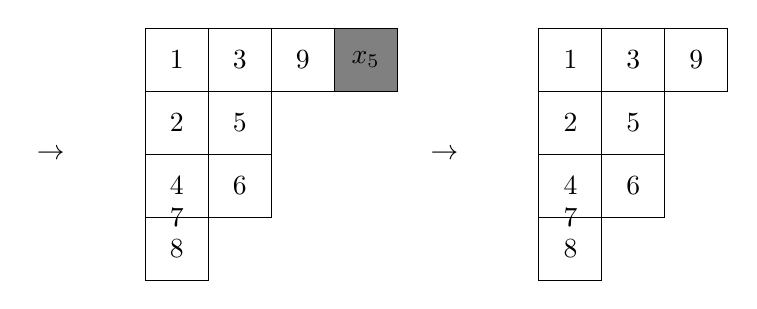
\begin{tikzpicture}
      \begin{scope}
        \fill[gray] (2.4,0) rectangle (3.2,-0.8);
        \draw (0,0)--(0,-3.2)--(0.8,-3.2)--(0.8,-2.4)--(1.6,-2.4)--(1.6,-0.8)--(3.2,-0.8)--(3.2,0)--cycle;
        \draw (0,-0.8)--(2.4,-0.8);
        \draw (0,-1.6)--(1.6,-1.6);
        \draw (0,-2.4)--(0.8,-2.4);
        \draw (0.8,0)--(0.8,-2.4);
        \draw (1.6,0)--(1.6,-2.4);
        \draw (2.4,0)--(2.4,-0.8);
  
        \node at (2,-0.4) {$9$};
        \node at (2.8,-0.4) {$x_5$};
        \node at (1.2,-2) {$6$};
        \node at (0.4,-2.8) {$8$};
  
        \node at (1.2,-1.2) {$5$};
        
        \node at (1.2,-0.4) {$3$};
        \node at (0.4,-2) {$4$};
        \node at (0.4,-2.4) {$7$};
        \node at (0.4,-1.2) {$2$};
        \node at (0.4,-0.4) {$1$};
        
        \node at (-1.2,-1.6) {$\rightarrow $};
        \node at (3.8,-1.6) {$\rightarrow $};
      \end{scope}
      \begin{scope}[xshift=5cm]
        \draw (0,0)--(0,-3.2)--(0.8,-3.2)--(0.8,-2.4)--(1.6,-2.4)--(1.6,-0.8)--(2.4,-0.8)--(2.4,0)--cycle;
        \draw (0,-0.8)--(2.4,-0.8);
        \draw (0,-1.6)--(1.6,-1.6);
        \draw (0,-2.4)--(0.8,-2.4);
        \draw (0.8,0)--(0.8,-2.4);
        \draw (1.6,0)--(1.6,-2.4);
        \draw (2.4,0)--(2.4,-0.8);
  
        \node at (2,-0.4) {$9$};
        \node at (1.2,-2) {$6$};
        \node at (0.4,-2.8) {$8$};
  
        \node at (1.2,-1.2) {$5$};
        
        \node at (1.2,-0.4) {$3$};
        \node at (0.4,-2) {$4$};
        \node at (0.4,-2.4) {$7$};
        \node at (0.4,-1.2) {$2$};
        \node at (0.4,-0.4) {$1$};
      \end{scope}
    \end{tikzpicture}
    \caption{図\ref{eg of 4331/221}左のtableauxのrectification.}\label{rect of 4331/221}
  \end{figure}
  \end{eg}

次に$T\in\text{EdSYT}(\mu/\lambda, n)$に対してそのウェイトを定義する.

\begin{defin}
  正の整数$m, k$を固定する.$\Lambda=\overbrace{(m,\cdots,m)}^{k\text{-copies}}$とする.$\Lambda$の箱$x$に対して
  \[
  \beta(x)=y_{i+1}-y_i\in \integer[y_1,\cdots,y_{m+k}]
  \]
  とする.ここで$i$は$\Lambda$の右上の隅の箱から$x$までのManhattan距離である(図\ref{manhattan}).
  \[
  \begin{ytableau}
    4 & 3 & 2 & 1\\
    5 & 4 & 3 & 2\\
    6 & 5 & 4 & 3
  \end{ytableau}
  \]
  \begin{figure}[H]
    \centering
    \caption{$k=3,m=4$における$\Lambda$の各箱のManhattan距離.}\label{manhattan}
  \end{figure}
\end{defin}

\begin{defin}
  $T\in\text{EqSYT}(\mu/\lambda, n), (\mu\leq\Lambda=\overbrace{(m,\cdots,m)}^{k\text{-copies}})$を固定し,$l$を$T$の辺のラベルに含まれる要素とする.$\text{factor}(l)\in\integer[y_1,\cdots,y_{m+k}]$を次のように定義する.$\text{EqRect}(T)$を計算する過程において,
  \begin{enumerate}
    \item $l$が含まれる列にある$\lambda$の箱をすべてequivariant jeu de taquinしたあとも,$l$が辺のラベルであるなら$\text{factor}(l)=0$とする.また$l$が含まれる列に$\lambda$の箱がない場合も$\text{factor}(l)=0$とする.
    \item $l$が含まれる列にある$\lambda$の箱をすべてequivariant jeu de taquinするとき,$l$が通った箱を下から順に$x_1,\cdots,x_s$とする.$x_s$と同じ行で$x_s$の右側にある$T$の箱を左から順に$y_1,\cdots,y_t$とする.このとき$\text{factor}(l)=\beta(x_1)+\cdots+\beta(x_s)+\beta(y_1)+\cdots+\beta(y_t)$とする.
  \end{enumerate}
\end{defin}

\begin{defin}
  $T\in\text{EqSYT}(\mu/\lambda, n)$に対して
  \[
  \text{wt}(T)=\prod_{l:\text{ edge label}}\text{factor}(l)
  \]
  とする.
\end{defin}

\begin{eg}
  例\ref{fst calculation}の計算より,
  \begin{center}
    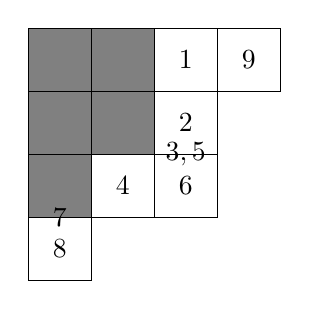
\begin{tikzpicture}
      \fill[gray] (0,0)--(1.6,0)--(1.6,-1.6)--(0.8,-1.6)--(0.8,-2.4)--(0,-2.4)--cycle;
        \draw (0,0)--(0,-3.2)--(0.8,-3.2)--(0.8,-2.4)--(2.4,-2.4)--(2.4,-0.8)--(3.2,-0.8)--(3.2,0)--cycle;
        \draw (0,-0.8)--(2.4,-0.8);
        \draw (0,-1.6)--(2.4,-1.6);
        \draw (0,-2.4)--(0.8,-2.4);
        \draw (0.8,0)--(0.8,-2.4);
        \draw (1.6,0)--(1.6,-2.4);
        \draw (2.4,0)--(2.4,-0.8);
  
        \node at (2,-0.4) {$1$};
        \node at (2.8,-0.4) {$9$};
        \node at (2,-1.2) {$2$};
        \node at (1.2,-2) {$4$};
        \node at (2,-2) {$6$};
        \node at (0.4,-2.8) {$8$};
  
        \node at (0.4,-2.4) {$7$};
        \node at (2,-1.6) {$3,5$};
    \end{tikzpicture}
  \end{center}
  のウェイトは
  \[
  \text{factor}(3)=\text{factor}(5)=\text{factor}(7)=0
  \]
  より$0$である.
\end{eg}

\begin{eg}
  図\ref{eg of 4331/221}右のtableauxのequivariant rectificationを図示する(図\ref{rect of 442}).
  \begin{figure}[H]
    \centering
    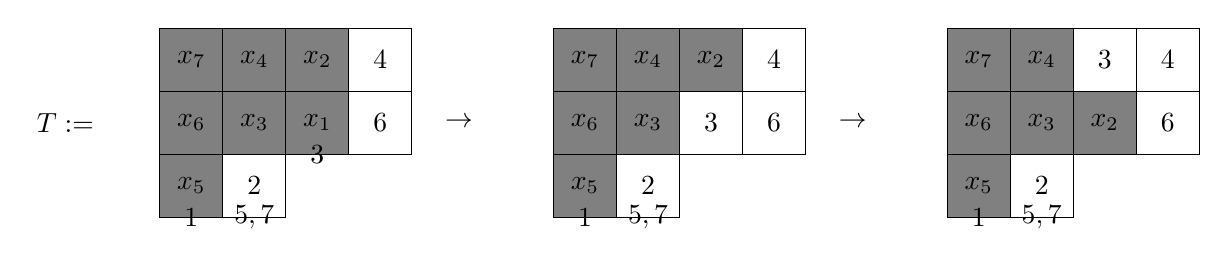
\begin{tikzpicture}
      \begin{scope}
        \fill[gray] (0,0)--(2.4,0)--(2.4,-1.6)--(0.8,-1.6)--(0.8,-2.4)--(0,-2.4)--cycle;
        \draw (0,0)--(3.2,0)--(3.2,-1.6)--(1.6,-1.6)--(1.6,-2.4)--(0,-2.4)--cycle;
        \draw (0.8,0)-- +(0,-2.4);
        \draw (1.6,0)-- +(0,-1.6);
        \draw (2.4,0)-- +(0,-1.6);
        \draw (0,-0.8)-- +(3.2,0);
        \draw (0,-1.6)-- +(1.6,0);
  
        \node at (2.8,-0.4) {$4$};
        \node at (2.8,-1.2) {$6$};
        \node at (1.2,-2) {$2$};
        \node at (0.4,-2.4) {$1$};
        \node at (1.2,-2.4) {$5,7$};
        \node at (2,-1.6) {$3$};

        \node at (2,-1.2) {$x_1$};
        \node at (2,-0.4) {$x_2$};
        \node at (1.2,-1.2) {$x_3$};
        \node at (1.2,-0.4) {$x_4$};
        \node at (0.4,-2) {$x_5$};
        \node at (0.4,-1.2) {$x_6$};
        \node at (0.4,-0.4) {$x_7$};

        \node at (-1.2,-1.2) {$T:=$};
        \node at (3.8,-1.2) {$\rightarrow $};
      \end{scope}
      \begin{scope}[xshift=5cm]
        \fill[gray] (0,0)--(2.4,0)--(2.4,-0.8)--(1.6,-0.8)--(1.6,-1.6)--(0.8,-1.6)--(0.8,-2.4)--(0,-2.4)--cycle;
        \draw (0,0)--(3.2,0)--(3.2,-1.6)--(1.6,-1.6)--(1.6,-2.4)--(0,-2.4)--cycle;
        \draw (0.8,0)-- +(0,-2.4);
        \draw (1.6,0)-- +(0,-1.6);
        \draw (2.4,0)-- +(0,-1.6);
        \draw (0,-0.8)-- +(3.2,0);
        \draw (0,-1.6)-- +(1.6,0);
  
        \node at (2.8,-0.4) {$4$};
        \node at (2.8,-1.2) {$6$};
        \node at (1.2,-2) {$2$};
        \node at (0.4,-2.4) {$1$};
        \node at (1.2,-2.4) {$5,7$};

        \node at (2,-1.2) {$3$};
        \node at (2,-0.4) {$x_2$};
        \node at (1.2,-1.2) {$x_3$};
        \node at (1.2,-0.4) {$x_4$};
        \node at (0.4,-2) {$x_5$};
        \node at (0.4,-1.2) {$x_6$};
        \node at (0.4,-0.4) {$x_7$};

        \node at (3.8,-1.2) {$\rightarrow $};
      \end{scope}
      \begin{scope}[xshift=10cm]
        \fill[gray] (0,0)--(1.6,0)--(1.6,-1.6)--(0.8,-1.6)--(0.8,-2.4)--(0,-2.4)--cycle;
        \fill[gray] (1.6,-0.8) rectangle (2.4,-1.6);
        \draw (0,0)--(3.2,0)--(3.2,-1.6)--(1.6,-1.6)--(1.6,-2.4)--(0,-2.4)--cycle;
        \draw (0.8,0)-- +(0,-2.4);
        \draw (1.6,0)-- +(0,-1.6);
        \draw (2.4,0)-- +(0,-1.6);
        \draw (0,-0.8)-- +(3.2,0);
        \draw (0,-1.6)-- +(1.6,0);
  
        \node at (2.8,-0.4) {$4$};
        \node at (2.8,-1.2) {$6$};
        \node at (1.2,-2) {$2$};
        \node at (0.4,-2.4) {$1$};
        \node at (1.2,-2.4) {$5,7$};

        \node at (2,-1.2) {$x_2$};
        \node at (2,-0.4) {$3$};
        \node at (1.2,-1.2) {$x_3$};
        \node at (1.2,-0.4) {$x_4$};
        \node at (0.4,-2) {$x_5$};
        \node at (0.4,-1.2) {$x_6$};
        \node at (0.4,-0.4) {$x_7$};
      \end{scope}
    \end{tikzpicture}

    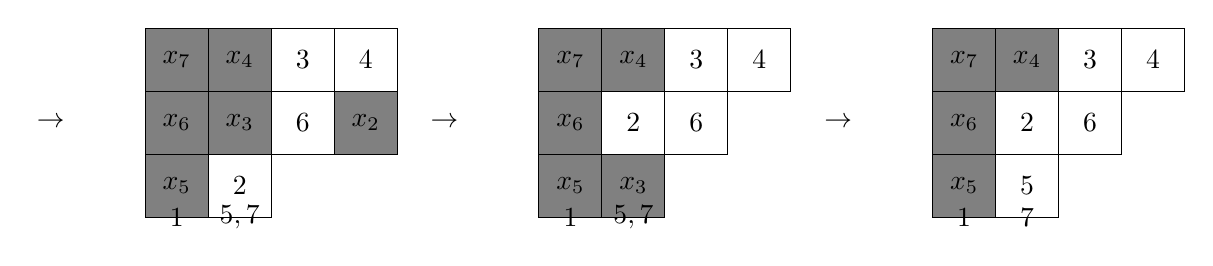
\begin{tikzpicture}
      \begin{scope}
        \fill[gray] (0,0)--(1.6,0)--(1.6,-1.6)--(0.8,-1.6)--(0.8,-2.4)--(0,-2.4)--cycle;
        \fill[gray] (2.4,-0.8) rectangle (3.2,-1.6);
        \draw (0,0)--(3.2,0)--(3.2,-1.6)--(1.6,-1.6)--(1.6,-2.4)--(0,-2.4)--cycle;
        \draw (0.8,0)-- +(0,-2.4);
        \draw (1.6,0)-- +(0,-1.6);
        \draw (2.4,0)-- +(0,-1.6);
        \draw (0,-0.8)-- +(3.2,0);
        \draw (0,-1.6)-- +(1.6,0);
  
        \node at (2.8,-0.4) {$4$};
        \node at (2.8,-1.2) {$x_2$};
        \node at (1.2,-2) {$2$};
        \node at (0.4,-2.4) {$1$};
        \node at (1.2,-2.4) {$5,7$};

        \node at (2,-1.2) {$6$};
        \node at (2,-0.4) {$3$};
        \node at (1.2,-1.2) {$x_3$};
        \node at (1.2,-0.4) {$x_4$};
        \node at (0.4,-2) {$x_5$};
        \node at (0.4,-1.2) {$x_6$};
        \node at (0.4,-0.4) {$x_7$};

        \node at (-1.2,-1.2) {$\rightarrow $};
        \node at (3.8,-1.2) {$\rightarrow $};
      \end{scope}
      \begin{scope}[xshift=5cm]
        \fill[gray] (0,0)--(1.6,0)--(1.6,-0.8)--(0.8,-0.8)--(0.8,-2.4)--(0,-2.4)--cycle;
        \fill[gray] (0.8,-1.6) rectangle (1.6,-2.4);
        \draw (0,0)--(3.2,0)--(3.2,-0.8)--(2.4,-0.8)--(2.4,-1.6)--(1.6,-1.6)--(1.6,-2.4)--(0,-2.4)--cycle;
        \draw (0.8,0)-- +(0,-2.4);
        \draw (1.6,0)-- +(0,-1.6);
        \draw (2.4,0)-- +(0,-1.6);
        \draw (0,-0.8)-- +(3.2,0);
        \draw (0,-1.6)-- +(1.6,0);
  
        \node at (2.8,-0.4) {$4$};
        \node at (1.2,-2) {$x_3$};
        \node at (0.4,-2.4) {$1$};
        \node at (1.2,-2.4) {$5,7$};

        \node at (2,-1.2) {$6$};
        \node at (2,-0.4) {$3$};
        \node at (1.2,-1.2) {$2$};
        \node at (1.2,-0.4) {$x_4$};
        \node at (0.4,-2) {$x_5$};
        \node at (0.4,-1.2) {$x_6$};
        \node at (0.4,-0.4) {$x_7$};

        \node at (3.8,-1.2) {$\rightarrow $};
      \end{scope}
      \begin{scope}[xshift=10cm]
        \fill[gray] (0,0)--(1.6,0)--(1.6,-0.8)--(0.8,-0.8)--(0.8,-2.4)--(0,-2.4)--cycle;
        \draw (0,0)--(3.2,0)--(3.2,-0.8)--(2.4,-0.8)--(2.4,-1.6)--(1.6,-1.6)--(1.6,-2.4)--(0,-2.4)--cycle;
        \draw (0.8,0)-- +(0,-2.4);
        \draw (1.6,0)-- +(0,-1.6);
        \draw (2.4,0)-- +(0,-1.6);
        \draw (0,-0.8)-- +(3.2,0);
        \draw (0,-1.6)-- +(1.6,0);
  
        \node at (2.8,-0.4) {$4$};
        \node at (1.2,-2) {$5$};
        \node at (0.4,-2.4) {$1$};
        \node at (1.2,-2.4) {$7$};

        \node at (2,-1.2) {$6$};
        \node at (2,-0.4) {$3$};
        \node at (1.2,-1.2) {$2$};
        \node at (1.2,-0.4) {$x_4$};
        \node at (0.4,-2) {$x_5$};
        \node at (0.4,-1.2) {$x_6$};
        \node at (0.4,-0.4) {$x_7$};
      \end{scope}
    \end{tikzpicture}

    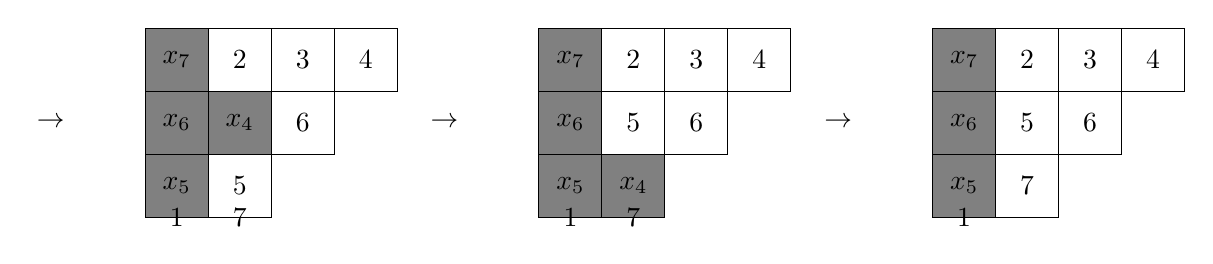
\begin{tikzpicture}
      \begin{scope}
        \fill[gray] (0,0)--(0.8,0)--(0.8,-2.4)--(0,-2.4)--cycle;
        \fill[gray] (0.8,-0.8) rectangle (1.6,-1.6);
        \draw (0,0)--(3.2,0)--(3.2,-0.8)--(2.4,-0.8)--(2.4,-1.6)--(1.6,-1.6)--(1.6,-2.4)--(0,-2.4)--cycle;
        \draw (0.8,0)-- +(0,-2.4);
        \draw (1.6,0)-- +(0,-1.6);
        \draw (2.4,0)-- +(0,-1.6);
        \draw (0,-0.8)-- +(3.2,0);
        \draw (0,-1.6)-- +(1.6,0);
  
        \node at (2.8,-0.4) {$4$};
        \node at (1.2,-2) {$5$};
        \node at (0.4,-2.4) {$1$};
        \node at (1.2,-2.4) {$7$};

        \node at (2,-1.2) {$6$};
        \node at (2,-0.4) {$3$};
        \node at (1.2,-1.2) {$x_4$};
        \node at (1.2,-0.4) {$2$};
        \node at (0.4,-2) {$x_5$};
        \node at (0.4,-1.2) {$x_6$};
        \node at (0.4,-0.4) {$x_7$};

        \node at (-1.2,-1.2) {$\rightarrow $};
        \node at (3.8,-1.2) {$\rightarrow $};
      \end{scope}
      \begin{scope}[xshift=5cm]
        \fill[gray] (0,0)--(0.8,0)--(0.8,-2.4)--(0,-2.4)--cycle;
        \fill[gray] (0.8,-1.6) rectangle (1.6,-2.4);
        \draw (0,0)--(3.2,0)--(3.2,-0.8)--(2.4,-0.8)--(2.4,-1.6)--(1.6,-1.6)--(1.6,-2.4)--(0,-2.4)--cycle;
        \draw (0.8,0)-- +(0,-2.4);
        \draw (1.6,0)-- +(0,-1.6);
        \draw (2.4,0)-- +(0,-1.6);
        \draw (0,-0.8)-- +(3.2,0);
        \draw (0,-1.6)-- +(1.6,0);
  
        \node at (2.8,-0.4) {$4$};
        \node at (1.2,-2) {$x_4$};
        \node at (0.4,-2.4) {$1$};
        \node at (1.2,-2.4) {$7$};

        \node at (2,-1.2) {$6$};
        \node at (2,-0.4) {$3$};
        \node at (1.2,-1.2) {$5$};
        \node at (1.2,-0.4) {$2$};
        \node at (0.4,-2) {$x_5$};
        \node at (0.4,-1.2) {$x_6$};
        \node at (0.4,-0.4) {$x_7$};

        \node at (3.8,-1.2) {$\rightarrow $};
      \end{scope}
      \begin{scope}[xshift=10cm]
        \fill[gray] (0,0)--(0.8,0)--(0.8,-2.4)--(0,-2.4)--cycle;
        \draw (0,0)--(3.2,0)--(3.2,-0.8)--(2.4,-0.8)--(2.4,-1.6)--(1.6,-1.6)--(1.6,-2.4)--(0,-2.4)--cycle;
        \draw (0.8,0)-- +(0,-2.4);
        \draw (1.6,0)-- +(0,-1.6);
        \draw (2.4,0)-- +(0,-1.6);
        \draw (0,-0.8)-- +(3.2,0);
        \draw (0,-1.6)-- +(1.6,0);
  
        \node at (2.8,-0.4) {$4$};
        \node at (1.2,-2) {$7$};
        \node at (0.4,-2.4) {$1$};

        \node at (2,-1.2) {$6$};
        \node at (2,-0.4) {$3$};
        \node at (1.2,-1.2) {$5$};
        \node at (1.2,-0.4) {$2$};
        \node at (0.4,-2) {$x_5$};
        \node at (0.4,-1.2) {$x_6$};
        \node at (0.4,-0.4) {$x_7$};
      \end{scope}
    \end{tikzpicture}

    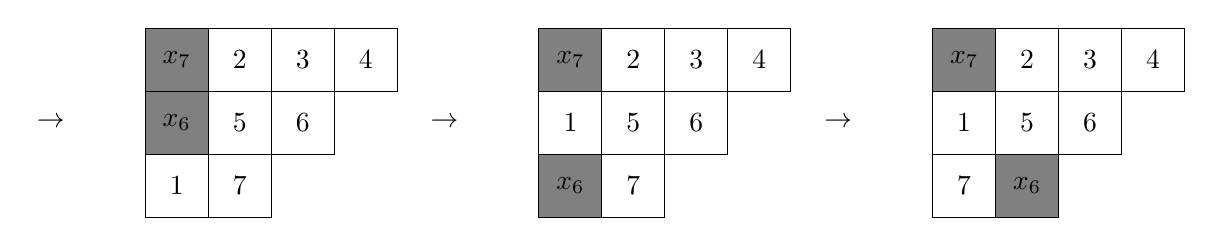
\begin{tikzpicture}
      \fill[gray] (0,0) rectangle (0.8,-1.6);
      \draw (0,0)--(3.2,0)--(3.2,-0.8)--(2.4,-0.8)--(2.4,-1.6)--(1.6,-1.6)--(1.6,-2.4)--(0,-2.4)--cycle;
      \draw (0.8,0)-- +(0,-2.4);
      \draw (1.6,0)-- +(0,-1.6);
      \draw (2.4,0)-- +(0,-1.6);
      \draw (0,-0.8)-- +(3.2,0);
      \draw (0,-1.6)-- +(1.6,0);

      \node at (2.8,-0.4) {$4$};
      \node at (1.2,-2) {$7$};
      \node at (2,-1.2) {$6$};
      \node at (2,-0.4) {$3$};
      \node at (1.2,-1.2) {$5$};
      \node at (1.2,-0.4) {$2$};
      \node at (0.4,-2) {$1$};
      \node at (0.4,-1.2) {$x_6$};
      \node at (0.4,-0.4) {$x_7$};

      \node at (-1.2,-1.2) {$\rightarrow $};
      \node at (3.8,-1.2) {$\rightarrow $};
      \begin{scope}[xshift=5cm]
        \fill[gray] (0,0) rectangle (0.8,-0.8);
        \fill[gray] (0,-1.6) rectangle (0.8,-2.4);
        \draw (0,0)--(3.2,0)--(3.2,-0.8)--(2.4,-0.8)--(2.4,-1.6)--(1.6,-1.6)--(1.6,-2.4)--(0,-2.4)--cycle;
        \draw (0.8,0)-- +(0,-2.4);
        \draw (1.6,0)-- +(0,-1.6);
        \draw (2.4,0)-- +(0,-1.6);
        \draw (0,-0.8)-- +(3.2,0);
        \draw (0,-1.6)-- +(1.6,0);

        \node at (2.8,-0.4) {$4$};
        \node at (1.2,-2) {$7$};
        \node at (2,-1.2) {$6$};
        \node at (2,-0.4) {$3$};
        \node at (1.2,-1.2) {$5$};
        \node at (1.2,-0.4) {$2$};
        \node at (0.4,-2) {$x_6$};
        \node at (0.4,-1.2) {$1$};
        \node at (0.4,-0.4) {$x_7$};

        \node at (3.8,-1.2) {$\rightarrow $};
      \end{scope}
      \begin{scope}[xshift=10cm]
        \fill[gray] (0,0) rectangle (0.8,-0.8);
        \fill[gray] (0.8,-1.6) rectangle (1.6,-2.4);
        \draw (0,0)--(3.2,0)--(3.2,-0.8)--(2.4,-0.8)--(2.4,-1.6)--(1.6,-1.6)--(1.6,-2.4)--(0,-2.4)--cycle;
        \draw (0.8,0)-- +(0,-2.4);
        \draw (1.6,0)-- +(0,-1.6);
        \draw (2.4,0)-- +(0,-1.6);
        \draw (0,-0.8)-- +(3.2,0);
        \draw (0,-1.6)-- +(1.6,0);

        \node at (2.8,-0.4) {$4$};
        \node at (1.2,-2) {$x_6$};
        \node at (2,-1.2) {$6$};
        \node at (2,-0.4) {$3$};
        \node at (1.2,-1.2) {$5$};
        \node at (1.2,-0.4) {$2$};
        \node at (0.4,-2) {$7$};
        \node at (0.4,-1.2) {$1$};
        \node at (0.4,-0.4) {$x_7$};
      \end{scope}
    \end{tikzpicture}

    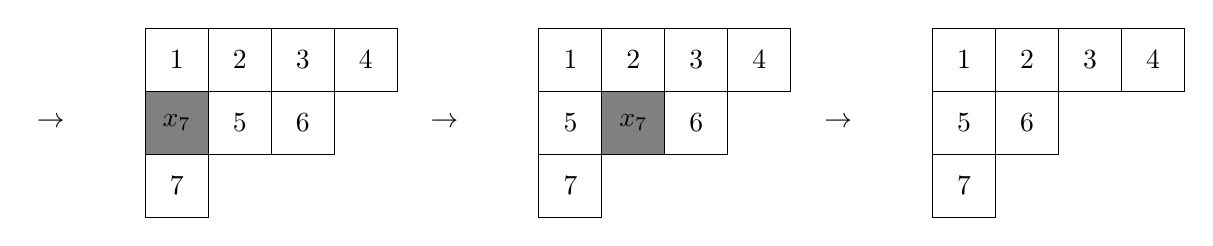
\begin{tikzpicture}
      \begin{scope}
        \fill[gray] (0,-0.8) rectangle (0.8,-1.6);
        \draw (0,0)--(3.2,0)--(3.2,-0.8)--(2.4,-0.8)--(2.4,-1.6)--(0.8,-1.6)--(0.8,-2.4)--(0,-2.4)--cycle;
        \draw (0.8,0)-- +(0,-2.4);
        \draw (1.6,0)-- +(0,-1.6);
        \draw (2.4,0)-- +(0,-1.6);
        \draw (0,-0.8)-- +(3.2,0);
        \draw (0,-1.6)-- +(1.6,0);

        \node at (2.8,-0.4) {$4$};
        \node at (2,-1.2) {$6$};
        \node at (2,-0.4) {$3$};
        \node at (1.2,-1.2) {$5$};
        \node at (1.2,-0.4) {$2$};
        \node at (0.4,-2) {$7$};
        \node at (0.4,-1.2) {$x_7$};
        \node at (0.4,-0.4) {$1$};

        \node at (-1.2,-1.2) {$\rightarrow $};
        \node at (3.8,-1.2) {$\rightarrow $};
      \end{scope}
      \begin{scope}[xshift=5cm]
        \fill[gray] (0.8,-0.8) rectangle (1.6,-1.6);
        \draw (0,0)--(3.2,0)--(3.2,-0.8)--(2.4,-0.8)--(2.4,-1.6)--(0.8,-1.6)--(0.8,-2.4)--(0,-2.4)--cycle;
        \draw (0.8,0)-- +(0,-2.4);
        \draw (1.6,0)-- +(0,-1.6);
        \draw (2.4,0)-- +(0,-1.6);
        \draw (0,-0.8)-- +(3.2,0);
        \draw (0,-1.6)-- +(1.6,0);

        \node at (2.8,-0.4) {$4$};
        \node at (2,-1.2) {$6$};
        \node at (2,-0.4) {$3$};
        \node at (1.2,-1.2) {$x_7$};
        \node at (1.2,-0.4) {$2$};
        \node at (0.4,-2) {$7$};
        \node at (0.4,-1.2) {$5$};
        \node at (0.4,-0.4) {$1$};

        \node at (3.8,-1.2) {$\rightarrow $};
      \end{scope}
      \begin{scope}[xshift=10cm]
        \draw (0,0)--(3.2,0)--(3.2,-0.8)--(1.6,-0.8)--(1.6,-1.6)--(0.8,-1.6)--(0.8,-2.4)--(0,-2.4)--cycle;
        \draw (0.8,0)-- +(0,-2.4);
        \draw (1.6,0)-- +(0,-1.6);
        \draw (2.4,0)-- +(0,-0.8);
        \draw (0,-0.8)-- +(3.2,0);
        \draw (0,-1.6)-- +(1.6,0);

        \node at (2.8,-0.4) {$4$};
        \node at (2,-0.4) {$3$};
        \node at (1.2,-1.2) {$6$};
        \node at (1.2,-0.4) {$2$};
        \node at (0.4,-2) {$7$};
        \node at (0.4,-1.2) {$5$};
        \node at (0.4,-0.4) {$1$};
      \end{scope}
    \end{tikzpicture}
    \caption{図\ref{eg of 4331/221}右のtableauxのrectification.}\label{rect of 442}
  \end{figure}
  $T\leq (4,4,4)$とみなして$\text{wt}(T)$を計算すると,上記の計算過程より
\begin{align*}
  &\text{factor}(3)=y_4-y_1\\
  &\text{factor}(5)=y_6-y_3\\
  &\text{factor}(7)=y_6-y_5\\
  &\text{factor}(1)=y_7-y_1\\
\end{align*}
  であるから
  \[
  \text{wt}(T)=(y_4-y_1)(y_6-y_3)(y_6-y_5)(y_7-y_1)
  \]
\end{eg}


分割$\mu$に対して,$1$行目の箱に左から順に$1,2,\cdots,\mu_1$を書き入れ,$2$行目の箱に左から順に$\mu_1+1,\mu_1+2,\cdots,\mu_1+\mu_2$を書き入れ,と続けて得られるstandard tableauxを$T_\mu$とする(図\ref{superstandard}).
\begin{figure}
  \centering
  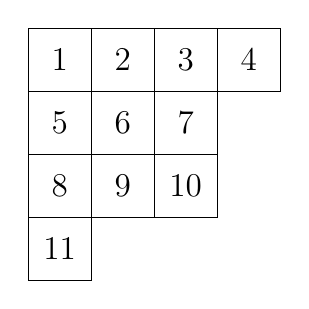
\begin{tikzpicture}
    \draw (0,0)-- ++(3.2,0)-- ++(0,-0.8)-- ++(-0.8,0)-- ++(0,-1.6)-- ++(-1.6,0)-- ++(0,-0.8)-- ++(-0.8,0)-- ++(0,3.2);
    \draw (0,-0.8)-- ++(2.4,0);
    \draw (0,-1.6)-- ++(2.4,0);
    \draw (0,-2.4)-- ++(0.8,0);
    \draw (0.8,0)-- ++(0,-2.4);
    \draw (1.6,0)-- ++(0,-2.4);
    \draw (2.4,0)-- ++(0,-0.8);

    \foreach \x in {1,2,3,4} {
      \node[font=\large] at (0.8 * \x - 0.4, -0.4) {$\x$};
    };
    \foreach \x in {5,6,7} {
      \node[font=\large] at (0.8 * \x - 3.6, -1.2) {$\x$};
    };
    \foreach \x in {8,9,10} {
      \node[font=\large] at (0.8 * \x - 6, -2) {$\x$};
    };
    \node[font=\large] at (0.4,-2.8) {$11$};
  \end{tikzpicture}
  \caption{$T_{(4,3,3,1)}$の図示.}\label{superstandard}
\end{figure}

正の整数$m,k$を固定する.分割$\lambda\leq\Lambda=\overbrace{(m,\cdots,m)}^{k\text{-copies}}$に対して,
\[
i_a=m-\lambda_a+a,\quad \text{for }a=1,\cdots,k
\]
とすると$i_1<\cdots<i_k$である.$l\in\binom{m+k}{k}$を,左から数えて$i_1,\cdots,i_k$番目に$1$が現れ,それ以外はすべて$0$であるような文字列とする.$\lambda$と$l$を対応させることで$\binom{m+k}{k}$と$\lambda\leq\Lambda$を満たす分割$\lambda$の集合を同一視する.

式(\ref{LRcoeff})の係数$C^\nu_{\lambda\mu}$に関して次が成り立つ.

\begin{theo}(Thomas-Yong \cite{thomas yong})
  \[
  C^{\nu}_{\lambda,\mu}=\sum_{\substack{T\in\text{EqSYT}(\nu/\lambda, |\mu|) \\ \text{EqRect}(T)=T_\mu \\ \text{wt}(T)\neq 0}}\text{wt}(T)
  \]
  が成り立つ.
\end{theo}




\subsection{weight preserving bijectionの構成}

このセクションではセクション3.3と3.4で構成した計算方法が,本質的に同じものであることを証明する.すなわち,$\mathcal{P}^\nu_{\lambda\mu}=\set{P:\text{puzzle}}{\partial P = \Delta^\nu_{\lambda\mu}}$,$\mathcal{T}^\nu_{\lambda\mu}=\set{T\in\text{EqSYT(\nu/\lambda,|\mu|)}}{\text{EqRect}(T)=T_\mu,\: \text{wt}(T)\neq 0}$とするとき,全単射$\varphi\colon \mathcal{P}^\nu_{\lambda\mu}\rightarrow \mathcal{T}^\nu_{\lambda\mu}$であって次の性質を満たすものを構成する.
\begin{equation}
  \text{wt}(\varphi(P))=\text{wt}(P)\quad\text{for all }P\in\mathcal{P}^\nu_{\lambda\mu}
\end{equation}

$\lambda,\mu,\nu\in\binom{n}{k}$とする.puzzle $P\in\mathcal{P}^\nu_{\lambda\mu}$は一般に図\ref{generic puzzle}の形をしている(\cite{Kreiman}).

\begin{figure}
  \centering
  \documentclass{ltjsarticle}
\RequirePackage{luatex85}
\usepackage[utf8]{inputenc}
\usepackage[dvipdfmx]{color}
\usepackage{enumerate}
\usepackage{here}
\usepackage{amsthm}
\usepackage{amsfonts}
\usepackage{amsmath}
\usepackage{amssymb}
\usepackage{latexsym}
\usepackage{ytableau}
\usepackage{docmute}
\usepackage{mathtools}
\usepackage{xr}
\usepackage{tikz}
\usetikzlibrary{intersections, calc, arrows.meta}
\usepackage[all]{xy}
\usepackage{graphics}
\usepackage[luatex]{hyperref}
%\usepackage{pxjahyper}



\theoremstyle{definition}
\newtheorem{defin}{定義}[subsection]
\newtheorem{theo}[defin]{定理}
\newtheorem{cor}[defin]{系}
\newtheorem{prop}[defin]{命題}
\newtheorem{lemm}[defin]{補題}
\newtheorem{notice}[defin]{注意}
\newtheorem{eg}[defin]{例}
\newtheorem{fact}[defin]{事実}


\renewcommand{\labelenumi}{(\roman{enumi})}


\newcommand{\invlimit}{\mathop{\lim_{\longleftarrow}}}
\newcommand{\dirlimit}{\mathop{\lim_{\longrightarrow}}}
\newcommand{\ind}{\text{Ind}}
\newcommand{\Hom}{\text{Hom}}
\newcommand{\tr}{\text{tr}}
\newcommand{\id}[1]{\text{id}_{#1}}
\newcommand{\sgn}{\mathrm{sgn}}
\newcommand{\res}[1]{\text{Res}_{#1}}
\newcommand{\generated}[1]{\langle\:#1\:\rangle}
\newcommand{\im}{\text{Im }}
\newcommand{\rank}{\text{rank }}
\newcommand{\del}[2]{\frac{\partial #1}{\partial #2}}
\newcommand{\delsametwo}[2]{\frac{\partial^2 #1}{\partial #2^2}}
\newcommand{\delothertwo}[3]{\frac{\partial^2#1}{\partial#2\partial#3}}
\newcommand{\ddel}[2]{\frac{\partial}{\partial #2}#1}
\newcommand{\ddelsametwo}[3]{\frac{\partial^2}{\partial #2^2}#1}
\newcommand{\ddelothertwo}[3]{\frac{\partial^2}{\partial#2\partial#3}#1}
\newcommand{\simneq}{\not\simeq}
\newcommand{\transpose}[1]{^t\!#1}
\newcommand{\ie}{\text{i.e.}}
\newcommand{\inv}[1]{#1^{-1}}
\newcommand{\real}{\mathbb{R}}
\newcommand{\complex}{\mathbb{C}}
\newcommand{\integer}{\mathbb{Z}}
\newcommand{\quotient}{\mathbb{Q}}
\newcommand{\natnum}{\mathbb{N}}
\newcommand{\proj}{\mathbb{P}}
\newcommand{\affine}{\mathbb{A}}
\newcommand{\tensor}[3]{#1\otimes_#2#3}
\newcommand{\map}[3]{#1:#2\rightarrow#3}
\newcommand{\aut}[2]{\mathrm{Aut}_{#1} (#2)}
\newcommand{\hommoph}[2]{\mathrm{Hom}_{#1}(#2)}
\newcommand{\gl}{\text{GL}}
\newcommand{\End}{\text{End}}
\newcommand{\set}[2]{\left\{\:#1\:\middle|\:#2\:\right\}}
\newcommand{\pmat}[1]{\begin{pmatrix} #1
\end{pmatrix}}
\newcommand{\vmat}[1]{\begin{vmatrix} #1
\end{vmatrix}}
\newcommand{\bmat}[1]{\begin{bmatrix} #1
\end{bmatrix}}
\newcommand{\br}{\vskip\baselineskip}
\newcommand{\Lie}{\text{Lie}}
\newcommand{\Sym}{\text{Sym}}
\newcommand{\Alt}{\text{Alt}}
\newcommand{\ch}{\text{ch}}
\newcommand{\diag}{\text{diag}}
\newcommand{\comb}[2]{_{#1}C_{#2}}
\newcommand{\codim}{\text{codim}\:}
\newcommand{\yd}[1]{\ydiagram{#1}}

\title{aaa}
\author{}
\date{}


\begin{document}
\maketitle

  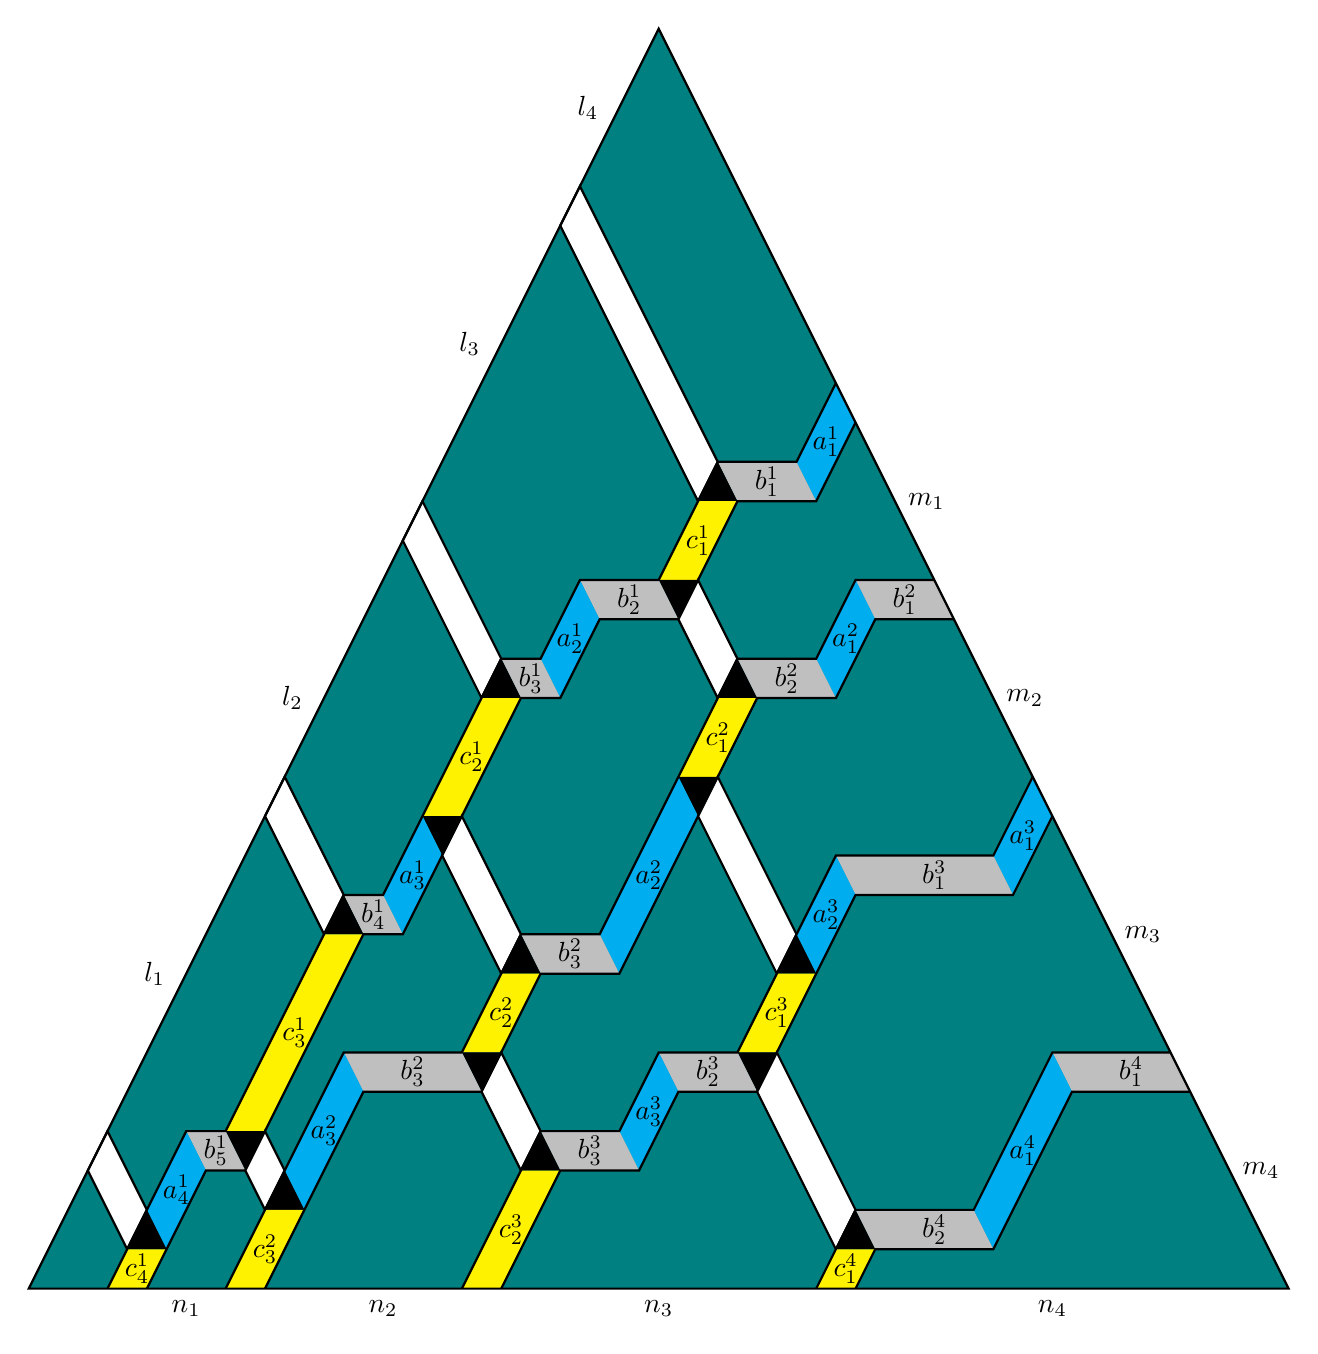
\begin{tikzpicture}
    \fill[teal] (0,0)--(16,0)--(8,16)--cycle;



    \fill[white] (3/4, 3/2)-- ++(2/4,-2/2)-- ++(1/4,1/2)-- ++(-2/4,2/2)--cycle;
    \draw[thick] (3/4, 3/2)-- ++(2/4,-2/2)-- ++(1/4,1/2)-- ++(-2/4,2/2)--cycle;

    \fill[white] (12/4, 12/2)-- ++(3/4,-3/2)-- ++(1/4,1/2)-- ++(-3/4,3/2)--cycle;
    \draw[thick] (12/4, 12/2)-- ++(3/4,-3/2)-- ++(1/4,1/2)-- ++(-3/4,3/2)--cycle;

    \fill[white] (19/4, 19/2)-- ++(4/4,-4/2)-- ++(1/4,1/2)-- ++(-4/4,4/2)--cycle;
    \draw[thick] (19/4, 19/2)-- ++(4/4,-4/2)-- ++(1/4,1/2)-- ++(-4/4,4/2)--cycle;

    \fill[white] (27/4, 27/2)-- ++(7/4,-7/2)-- ++(1/4,1/2)-- ++(-7/4,7/2)--cycle;
    \draw[thick] (27/4, 27/2)-- ++(7/4,-7/2)-- ++(1/4,1/2)-- ++(-7/4,7/2)--cycle;

    \fill[cyan] (8+9/4,16-9/2)-- ++(-2/4,-2/2)-- ++(1/4,-1/2)-- ++(2/4,2/2)--cycle;
    \node at (8+8/4+1/8,16-10/2-1/4) {$a^1_1$};
    \fill[lightgray] (8+7/4,16-11/2)-- ++(-1,0)-- ++(1/4,-1/2)-- ++(1,0)--cycle;
    \node at (8+6/4-1/8,16-11/2-1/4) {$b^1_1$};
    \fill[black] (8+3/4,16-11/2)-- ++(-1/4,-1/2)-- ++(1/2,0)--cycle;
    \fill[yellow] (8+2/4,16-12/2)-- ++(-2/4,-2/2)-- ++(1/2,0)-- ++(2/4,2/2)--cycle;
    \node at (8+1/4+2/8,16-13/2) {$c^1_1$};
    \fill[black] (8,16-14/2)-- ++(1/2,0)-- ++(-1/4,-1/2)--cycle;
    \fill[lightgray] (8,16-14/2)-- ++(-1,0)-- ++(1/4,-1/2)-- ++(1,0)--cycle;
    \node at (8-1/4-1/8,16-14/2-1/4) {$b^1_2$};
    \fill[cyan] (8-4/4,16-14/2)-- ++(-2/4,-2/2)-- ++(1/4,-1/2)-- ++(2/4,2/2)--cycle;
    \node at (8-5/4+1/8,16-15/2-1/4) {$a^1_2$};
    \fill[lightgray] (8-6/4, 16-16/2)-- ++(-1/2,0)-- ++(1/4,-1/2)-- ++(1/2,0)--cycle;
    \node at (8-7/4+1/8, 16-16/2-1/4) {$b^1_3$};
    \fill[black] (8-8/4,16-16/2)-- ++(-1/4,-1/2)-- ++(1/2,0)--cycle;
    \fill[yellow] (8-9/4, 16-17/2)-- ++(-3/4,-3/2)-- ++(1/2,0)-- ++(3/4,3/2)--cycle;
    \node at (8-10/4+1/8, 16-18/2-1/4) {$c^1_2$};
    \fill[black] (8-12/4,16-20/2)-- ++(1/2,0)-- ++(-1/4,-1/2)--cycle;
    %
    \fill[cyan] (8-12/4,16-20/2)-- ++(-1/2,-2/2)-- ++(1/4,-1/2)-- ++(1/2,2/2)--cycle;
    \node at (8-13/4+1/8,16-21/2-1/4) {$a^1_3$};
    \fill[lightgray] (8-14/4, 16-22/2)-- ++(-1/2,0)-- ++(1/4,-1/2)-- ++(1/2,0)--cycle;
    \node at (8-15/4+1/8, 16-22/2-1/4) {$b^1_4$};
    \fill[black] (8-16/4,16-22/2)-- ++(-1/4,-1/2)-- ++(1/2,0)--cycle;
    \fill[yellow] (8-17/4,16-23/2)-- ++(-5/4,-5/2)-- ++(1/2,0)-- ++(5/4,5/2)--cycle;
    \node at (8-19/4+1/8,16-25/2-1/4) {$c^1_3$};
    \fill[black] (8-22/4,16-28/2)-- ++(1/2,0)-- ++(-1/4,-1/2)--cycle;
    \fill[lightgray] (8-22/4,16-28/2)-- ++(-1/2,0)-- ++(1/4,-1/2)-- ++(1/2,0)--cycle;
    \node at (8-23/4+1/8,16-28/2-1/4) {$b^1_5$};
    \fill[cyan] (8-24/4,16-28/2)-- ++(-2/4,-2/2)-- ++(1/4,-1/2)-- ++(2/4,2/2)--cycle;
    \node at (8-24/4-1/8,16-29/2-1/4) {$a^1_4$};
    \fill[black] (8-26/4,16-30/2)-- ++(-1/4,-1/2)-- ++(1/2,0)--cycle;
    \fill[yellow] (8-27/4, 16-31/2)-- ++(-1/4,-1/2)-- ++(1/2,0)-- ++(1/4,1/2)--cycle;
    \node at (8-27/4+1/8, 16-31/2-1/4) {$c^1_4$};

    \draw[thick] (8+9/4,16-9/2)-- ++(-1/2, -1)-- ++(-1,0)-- ++(-3/4, -3/2)-- ++(-1,0)-- ++(-1/2,-1)-- ++(-1/2,0)-- ++(-3/2,-3)-- ++(-1/2,0)-- ++(-3/2,-3)-- ++(-1/2,0)-- ++(-1,-2);
    \draw[thick] (8+10/4,16-5)-- ++(-1/2,-1)-- ++(-1,0)-- ++(-3/4,-3/2)-- ++(-1,0)-- ++(-1/2,-1)-- ++(-1/2,0)-- ++(-3/2,-3)-- ++(-1/2,0)-- ++(-3/2,-3)-- ++(-1/2, 0)-- ++(-3/4,-3/2);



    \fill[white] (8+4/4, 16-16/2)-- ++(-2/4,2/2)-- ++(-1/4,-1/2)-- ++(2/4,-2/2)--cycle;
    \draw[thick] (8+4/4, 16-16/2)-- ++(-2/4,2/2)-- ++(-1/4,-1/2)-- ++(2/4,-2/2)--cycle;

    \fill[white] (8-7/4,16-23/2)-- ++(-3/4,3/2)-- ++(-1/4,-1/2)-- ++(3/4,-3/2)--cycle;
    \draw[thick] (8-7/4,16-23/2)-- ++(-3/4,3/2)-- ++(-1/4,-1/2)-- ++(3/4,-3/2)--cycle;

    \fill[white] (8-19/4,16-29/2)-- ++(-1/4,1/2)-- ++(-1/4,-1/2)-- ++(1/4,-1/2)--cycle;
    \draw[thick] (8-19/4,16-29/2)-- ++(-1/4,1/2)-- ++(-1/4,-1/2)-- ++(1/4,-1/2)--cycle;

    \fill[lightgray] (8+14/4,16-14/2)-- ++(-1,0)-- ++(1/4,-1/2)-- ++(1,0)--cycle;
    \node at (8+13/4-1/8,16-14/2-1/4) {$b^2_1$};
    \fill[cyan] (8+10/4,16-14/2)-- ++(-1/2,-1)-- ++(1/4,-1/2)-- ++(1/2,1)--cycle;
    \node at (8+9/4+1/8,16-15/2-1/4) {$a^2_1$};
    \fill[lightgray] (8+8/4,16-16/2)-- ++(-1,0)-- ++(1/4,-1/2)-- ++(1,0)--cycle;
    \node at (8+7/4-1/8,16-16/2-1/4) {$b^2_2$};
    \fill[black] (8+4/4, 16-16/2)-- ++(-1/4,-1/2)-- ++(1/2,0)--cycle;
    \fill[yellow] (8+3/4, 16-17/2)-- ++(-1/2,-1)-- ++(1/2,0)-- ++(1/2,1)--cycle;
    \node at (8+2/4+2/8, 16-18/2) {$c^2_1$};
    \fill[black] (8+1/4,16-19/2)-- ++(1/2,0)-- ++(-1/4,-1/2)--cycle;
    \fill[cyan] (8+1/4,16-19/2)-- ++(-1,-2)-- ++(1/4,-1/2)-- ++(1,2)--cycle;
    \node at  (8-1/4+1/8,16-21/2-1/4) {$a^2_2$};
    \fill[lightgray] (8-3/4,16-23/2)-- ++(-1,0)-- ++(1/4,-1/2)-- ++(1,0)--cycle;
    \node at (8-4/4-1/8,16-23/2-1/4) {$b^2_3$};
    \fill[black] (8-7/4,16-23/2)-- ++(-1/4,-1/2)-- ++(1/2,0)--cycle;
    \fill[yellow] (8-8/4,16-24/2)-- ++(-1/2,-1)-- ++(1/2,0)-- ++(1/2,1)--cycle;
    \node at (8-9/4+2/8,16-25/2) {$c^2_2$};
    \fill[black] (8-10/4,16-26/2)-- ++(1/2,0)-- ++(-1/4,-1/2)--cycle;
    \fill[lightgray] (8-10/4,16-26/2)-- ++(-3/2,0)-- ++(1/4,-1/2)-- ++(3/2,0)--cycle;
    \node at (8-12/4-1/8,16-26/2-1/4) {$b^2_3$};
    \fill[cyan] (8-16/4,16-26/2)-- ++(-3/4,-3/2)-- ++(1/4,-1/2)-- ++(3/4,3/2)--cycle;
    \node at (8-17/4,16-28/2) {$a^2_3$};
    \fill[black] (8-19/4,16-29/2)-- ++(-1/4,-1/2)-- ++(1/2,0)--cycle;
    \fill[yellow] (8-20/4,16-30/2)-- ++(-1/2,-1)-- ++(1/2,0)-- ++(1/2,1)--cycle;
    \node at (8-21/4+2/8,16-31/2) {$c^2_3$};

    \draw[thick] (8+14/4,16-14/2)-- ++(-1,0)-- ++(-1/2,-1)-- ++(-1,0)-- ++(-7/4,-7/2)-- ++(-1,0)-- ++(-3/4,-3/2)-- ++(-3/2,0)-- ++(-6/4,-6/2);
    \draw[thick] (8+15/4, 16-15/2)-- ++(-1,0)-- ++(-1/2,-1)-- ++(-1,0)-- ++(-7/4,-7/2)-- ++(-1,0)-- ++(-3/4,-3/2)-- ++(-3/2,0)-- ++(-5/4,-5/2);



    \fill[white] (8+7/4,16-23/2)-- ++(-1,2)-- ++(-1/4,-1/2)-- ++(1,-2)--cycle;
    \draw[thick] (8+7/4,16-23/2)-- ++(-1,2)-- ++(-1/4,-1/2)-- ++(1,-2)--cycle;

    \fill[white] (8-6/4,16-28/2)-- ++(-1/2,1)-- ++(-1/4,-1/2)-- ++(1/2,-1)--cycle;
    \draw[thick] (8-6/4,16-28/2)-- ++(-1/2,1)-- ++(-1/4,-1/2)-- ++(1/2,-1)--cycle;

    \fill[cyan] (8+19/4,16-19/2)-- ++(-1/2,-1)-- ++(1/4,-1/2)-- ++(1/2,1)--cycle;
    \node at (8+18/4+1/8,16-20/2-1/4) {$a^3_1$};
    \fill[lightgray] (8+17/4,16-21/2)-- ++(-2,0)-- ++(1/4,-1/2)-- ++(2,0)--cycle;
    \node at (8+14/4,16-21/2-1/4) {$b^3_1$};
    \fill[cyan] (8+9/4,16-21/2)-- ++(-2/4,-2/2)-- ++(1/4,-1/2)-- ++(2/4,2/2)--cycle;
    \node at (8+8/4+1/8,16-22/2-1/4) {$a^3_2$};
    \fill[black] (8+7/4,16-23/2)-- ++(-1/4,-1/2)-- ++(1/2,0)--cycle;
    \fill[yellow] (8+6/4,16-24/2)-- ++(-2/4,-2/2)-- ++(1/2,0)-- ++(1/2,1)--cycle;
    \node at (8+5/4+2/8,16-25/2) {$c^3_1$};
    \fill[black] (8+4/4,16-26/2)-- ++(1/2,0)-- ++(-1/4,-1/2)--cycle;
    \fill[lightgray] (8+4/4,16-26/2)-- ++(-1,0)-- ++(1/4,-1/2)-- ++(1,0)--cycle;
    \node at (8+3/4-1/8,16-26/2-1/4) {$b^3_2$};
    \fill[cyan] (8,16-26/2)-- ++(-1/2,-1)-- ++(1/4,-1/2)-- ++(1/2,1)--cycle;
    \node at (8-1/4+1/8,16-27/2-1/4) {$a^3_3$};
    \fill[lightgray] (8-2/4,16-28/2)-- ++(-1,0)-- ++(1/4,-1/2)-- ++(1,0)--cycle;
    \node at (8-3/4-1/8,16-28/2-1/4) {$b^3_3$};
    \fill[black] (8-6/4,16-28/2)-- ++(-1/4,-1/2)-- ++(1/2,0)--cycle;
    \fill[yellow] (8-7/4,16-29/2)-- ++(-3/4,-3/2)-- ++(1/2,0)-- ++(3/4,3/2)--cycle;
    \node at (8-8/4+1/8,16-30/2-1/4) {$c^3_2$};

    \draw[thick] (8+19/4,16-19/2)-- ++(-1/2,-1)-- ++(-2,0)-- ++(-5/4,-5/2)-- ++(-1,0)-- ++(-1/2,-1)-- ++(-1,0)-- ++(-1,-2);
    \draw[thick] (8+20/4,16-20/2)-- ++(-1/2,-1)-- ++(-2,0)-- ++(-5/4,-5/2)-- ++(-1,0)-- ++(-1/2,-1)-- ++(-1,0)-- ++(-3/4,-3/2);



    \fill[white] (8+10/4,16-30/2)-- ++(-1,2)-- ++(-1/4,-1/2)-- ++(1,-2)--cycle;
    \draw[thick] (8+10/4,16-30/2)-- ++(-1,2)-- ++(-1/4,-1/2)-- ++(1,-2)--cycle;

    \fill[lightgray] (8+26/4, 16-26/2)-- ++(-3/2,0)-- ++(1/4,-1/2)-- ++(3/2,0)--cycle;
    \node at (8+24/4, 16-26/2-1/4) {$b^4_1$};
    \fill[cyan] (8+20/4, 16-26/2)-- ++(-1,-2)-- ++(1/4,-1/2)-- ++(1,2)--cycle;
    \node at (8+18/4+1/8, 16-28/2-1/4) {$a^4_1$};
    \fill[lightgray] (8+16/4,16-30/2)-- ++(-3/2,0)-- ++(1/4,-1/2)-- ++(3/2,0)--cycle;
    \node at (8+14/4,16-30/2-1/4) {$b^4_2$};
    \fill[black] (8+10/4,16-30/2)-- ++(-1/4,-1/2)-- ++(1/2,0)--cycle;
    \fill[yellow] (8+9/4,16-31/2)-- ++(-1/4,-1/2)-- ++(1/2,0)-- ++(1/4,1/2)--cycle;
    \node at (8+9/4+1/8,16-31/2-1/4) {$c^4_1$};

    \draw[thick] (8+26/4, 16-26/2)-- ++(-3/2,0)-- ++(-1,-2)-- ++(-3/2,0)-- ++(-1/2,-1);
    \draw[thick] (8+27/4, 16-27/2)-- ++(-3/2,0)-- ++(-1,-2)-- ++(-3/2,0)-- ++(-1/4,-1/2);

    \draw[thick] (0,0)--(16,0)--(8,16)--cycle;

    \node at (-2/5 + 8/4, 8/2) {$l_1$};
    \node at (-2/5 + 15/4, 15/2) {$l_2$};
    \node at (-2/5 + 24/4, 24/2) {$l_3$};
    \node at (-2/5 + 30/4, 30/2) {$l_4$};

    \node at (2, -1/4) {$n_1$};
    \node at (9/2, -1/4) {$n_2$};
    \node at (16/2, -1/4) {$n_3$};
    \node at (26/2, -1/4) {$n_4$};

    \node at (16 + 2/5 - 3/4, 3/2) {$m_4$};
    \node at (16 + 2/5 - 9/4, 9/2) {$m_3$};
    \node at (16 + 2/5 - 15/4, 15/2) {$m_2$};
    \node at (16 + 2/5 - 20/4, 20/2) {$m_1$};
  \end{tikzpicture}

\end{document}
  \caption{puzzleの一般形\cite{Kreiman}.
  ここで,水色の領域は
  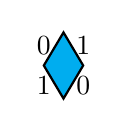
\begin{tikzpicture}[baseline=-1pt]
    \fill[cyan] (0,0)--(0.25,0.42)--(0.5,0)--(0.25,-0.42)--cycle;
    \protect\draw[thick] (0,0)--(0.25,0.42)--(0.5,0)--(0.25,-0.42)--cycle;
    \protect\node at (0,0.25) {$0$};
    \protect\node at (0.5,0.25) {$1$};
    \protect\node at (0,-0.25) {$1$};
    \protect\node at (0.5,-0.25) {$0$};
  \end{tikzpicture}
  ,灰色の領域は
  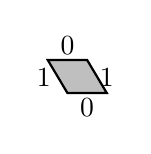
\begin{tikzpicture}[baseline=2pt]
    \fill[lightgray] (0,0)-- ++(0.5,0)-- ++(-0.25,0.42)-- ++(-0.5,0)--cycle;
    \protect\draw[thick](0,0)-- ++(0.5,0)-- ++(-0.25,0.42)-- ++(-0.5,0)--cycle;
    \protect\node at (-0.3,0.2) {$1$};
    \protect\node at (0.25,-0.18) {$0$};
    \protect\node at (0.5,0.2) {$1$};
    \protect\node at (0, 0.6) {$0$};
  \end{tikzpicture}
  ,黄色の領域は
  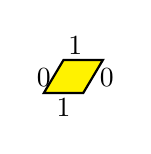
\begin{tikzpicture}[baseline=2pt]
    \fill[yellow] (0,0)-- ++(0.5,0)-- ++(0.25,0.42)-- ++(-0.5,0)--cycle;
    \protect\draw[thick](0,0)-- ++(0.5,0)-- ++(0.25,0.42)-- ++(-0.5,0)--cycle;
    \protect\node at (0,0.2) {$0$};
    \protect\node at (0.25,-0.18) {$1$};
    \protect\node at (0.8,0.2) {$0$};
    \protect\node at (0.4, 0.6) {$1$};
  \end{tikzpicture}
  ,白色の領域は
  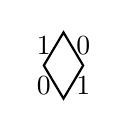
\begin{tikzpicture}[baseline=-1pt]
    \protect\draw[thick] (0,0)--(0.25,0.42)--(0.5,0)--(0.25,-0.42)--cycle;
    \protect\node at (0,0.25) {$1$};
    \protect\node at (0.5,0.25) {$0$};
    \protect\node at (0,-0.25) {$0$};
    \protect\node at (0.5,-0.25) {$1$};
  \end{tikzpicture}
  ,黒色の領域は
  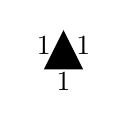
\begin{tikzpicture}[baseline=1pt]
    \fill[black] (0,0)-- ++(0.5,0)-- ++(-0.25,0.5)--cycle;
    \protect\node at (0,0.3) {$1$};
    \protect\node at (0.5,0.3) {$1$};
    \protect\node at (0.25,-0.15) {$1$};
  \end{tikzpicture}
  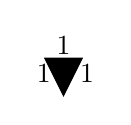
\begin{tikzpicture}[baseline=2pt]
    \fill[black] (0,0.5)-- ++(0.5,0)-- ++(-0.25,-0.5)--cycle;
    \protect\node at (0.25, 0.65) {$1$};
    \protect\node at (0,0.3) {$1$};
    \protect\node at (0.55,0.3) {$1$};
  \end{tikzpicture}
  ,緑色の領域は
  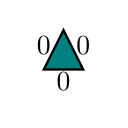
\begin{tikzpicture}[baseline=1pt]
    \fill[teal] (0,0)-- ++(0.5,0)-- ++(-0.25,0.5)--cycle;
    \protect\draw[thick] (0,0)-- ++(0.5,0)-- ++(-0.25,0.5)--cycle;
    \protect\node at (0,0.3) {$0$};
    \protect\node at (0.5,0.3) {$0$};
    \protect\node at (0.25,-0.15) {$0$};
  \end{tikzpicture}
  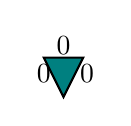
\begin{tikzpicture}[baseline=2pt]
    \fill[teal] (0,0.5)-- ++(0.5,0)-- ++(-0.25,-0.5)--cycle;
    \protect\draw[thick] (0,0.5)-- ++(0.5,0)-- ++(-0.25,-0.5)--cycle;
    \protect\node at (0.25, 0.65) {$0$};
    \protect\node at (0,0.3) {$0$};
    \protect\node at (0.55,0.3) {$0$};
  \end{tikzpicture}
  のそれぞれのからなり,$a^i_j, b^i_j, c^i_j$は各puzzle pieceの個数を表す.$l_i,m_i,n_i$はそれぞれの部分における$0$の個数である.
  }\label{generic puzzle}
\end{figure}


$P$の

\begin{tikzpicture}[baseline=-1pt]
  \fill[cyan] (0,0)--(0.25,0.42)--(0.5,0)--(0.25,-0.42)--cycle;
  \draw[thick] (0,0)--(0.25,0.42)--(0.5,0)--(0.25,-0.42)--cycle;
\end{tikzpicture}

\begin{tikzpicture}[baseline=2pt]
  \fill[lightgray] (0,0)-- ++(0.5,0)-- ++(-0.25,0.42)-- ++(-0.5,0)--cycle;
  \draw[thick](0,0)-- ++(0.5,0)-- ++(-0.25,0.42)-- ++(-0.5,0)--cycle;
\end{tikzpicture}

\begin{tikzpicture}[baseline=2pt]
  \fill[yellow] (0,0)-- ++(0.5,0)-- ++(0.25,0.42)-- ++(-0.5,0)--cycle;
  \draw[thick](0,0)-- ++(0.5,0)-- ++(0.25,0.42)-- ++(-0.5,0)--cycle;
\end{tikzpicture}

\begin{tikzpicture}[baseline=1pt]
  \fill[black] (0,0)-- ++(0.5,0)-- ++(-0.25,0.5)--cycle;
\end{tikzpicture}

\begin{tikzpicture}[baseline=2pt]
  \fill[black] (0,0.5)-- ++(0.5,0)-- ++(-0.25,-0.5)--cycle;
\end{tikzpicture}
のpuzzle pieceからなる連結領域をpath と呼び,

\begin{tikzpicture}[baseline=2pt]
  \fill[black] (0,0.5)-- ++(0.5,0)-- ++(-0.25,-0.5)--cycle;
\end{tikzpicture}
で挟まれた部分をsegmentと呼ぶ.またsegmentに含まれる

\begin{tikzpicture}[baseline=-1pt]
  \fill[cyan] (0,0)--(0.25,0.42)--(0.5,0)--(0.25,-0.42)--cycle;
  \draw[thick] (0,0)--(0.25,0.42)--(0.5,0)--(0.25,-0.42)--cycle;
\end{tikzpicture}

\begin{tikzpicture}[baseline=2pt]
  \fill[lightgray] (0,0)-- ++(0.5,0)-- ++(-0.25,0.42)-- ++(-0.5,0)--cycle;
  \draw[thick](0,0)-- ++(0.5,0)-- ++(-0.25,0.42)-- ++(-0.5,0)--cycle;
\end{tikzpicture}

\begin{tikzpicture}[baseline=2pt]
  \fill[yellow] (0,0)-- ++(0.5,0)-- ++(0.25,0.42)-- ++(-0.5,0)--cycle;
  \draw[thick](0,0)-- ++(0.5,0)-- ++(0.25,0.42)-- ++(-0.5,0)--cycle;
\end{tikzpicture}
のpuzzle pieceの個数をそのsegmentの長さと呼ぶ(図\ref{path,segment}).segment $s$に対してその長さを$|s|$と書く.

\begin{figure}
  \centering
  \documentclass{ltjsarticle}
\RequirePackage{luatex85}
\usepackage[utf8]{inputenc}
\usepackage[dvipdfmx]{color}
\usepackage{enumerate}
\usepackage{here}
\usepackage{amsthm}
\usepackage{amsfonts}
\usepackage{amsmath}
\usepackage{amssymb}
\usepackage{latexsym}
\usepackage{ytableau}
\usepackage{docmute}
\usepackage{mathtools}
\usepackage{xr}
\usepackage{tikz}
\usetikzlibrary{intersections, calc, arrows.meta}
\usepackage[all]{xy}
\usepackage{graphics}
\usepackage[luatex]{hyperref}
%\usepackage{pxjahyper}



\theoremstyle{definition}
\newtheorem{defin}{定義}[subsection]
\newtheorem{theo}[defin]{定理}
\newtheorem{cor}[defin]{系}
\newtheorem{prop}[defin]{命題}
\newtheorem{lemm}[defin]{補題}
\newtheorem{notice}[defin]{注意}
\newtheorem{eg}[defin]{例}
\newtheorem{fact}[defin]{事実}


\renewcommand{\labelenumi}{(\roman{enumi})}


\newcommand{\invlimit}{\mathop{\lim_{\longleftarrow}}}
\newcommand{\dirlimit}{\mathop{\lim_{\longrightarrow}}}
\newcommand{\ind}{\text{Ind}}
\newcommand{\Hom}{\text{Hom}}
\newcommand{\tr}{\text{tr}}
\newcommand{\id}[1]{\text{id}_{#1}}
\newcommand{\sgn}{\mathrm{sgn}}
\newcommand{\res}[1]{\text{Res}_{#1}}
\newcommand{\generated}[1]{\langle\:#1\:\rangle}
\newcommand{\im}{\text{Im }}
\newcommand{\rank}{\text{rank }}
\newcommand{\del}[2]{\frac{\partial #1}{\partial #2}}
\newcommand{\delsametwo}[2]{\frac{\partial^2 #1}{\partial #2^2}}
\newcommand{\delothertwo}[3]{\frac{\partial^2#1}{\partial#2\partial#3}}
\newcommand{\ddel}[2]{\frac{\partial}{\partial #2}#1}
\newcommand{\ddelsametwo}[3]{\frac{\partial^2}{\partial #2^2}#1}
\newcommand{\ddelothertwo}[3]{\frac{\partial^2}{\partial#2\partial#3}#1}
\newcommand{\simneq}{\not\simeq}
\newcommand{\transpose}[1]{^t\!#1}
\newcommand{\ie}{\text{i.e.}}
\newcommand{\inv}[1]{#1^{-1}}
\newcommand{\real}{\mathbb{R}}
\newcommand{\complex}{\mathbb{C}}
\newcommand{\integer}{\mathbb{Z}}
\newcommand{\quotient}{\mathbb{Q}}
\newcommand{\natnum}{\mathbb{N}}
\newcommand{\proj}{\mathbb{P}}
\newcommand{\affine}{\mathbb{A}}
\newcommand{\tensor}[3]{#1\otimes_#2#3}
\newcommand{\map}[3]{#1:#2\rightarrow#3}
\newcommand{\aut}[2]{\mathrm{Aut}_{#1} (#2)}
\newcommand{\hommoph}[2]{\mathrm{Hom}_{#1}(#2)}
\newcommand{\gl}{\text{GL}}
\newcommand{\End}{\text{End}}
\newcommand{\set}[2]{\left\{\:#1\:\middle|\:#2\:\right\}}
\newcommand{\pmat}[1]{\begin{pmatrix} #1
\end{pmatrix}}
\newcommand{\vmat}[1]{\begin{vmatrix} #1
\end{vmatrix}}
\newcommand{\bmat}[1]{\begin{bmatrix} #1
\end{bmatrix}}
\newcommand{\br}{\vskip\baselineskip}
\newcommand{\Lie}{\text{Lie}}
\newcommand{\Sym}{\text{Sym}}
\newcommand{\Alt}{\text{Alt}}
\newcommand{\ch}{\text{ch}}
\newcommand{\diag}{\text{diag}}
\newcommand{\comb}[2]{_{#1}C_{#2}}
\newcommand{\codim}{\text{codim}\:}
\newcommand{\yd}[1]{\ydiagram{#1}}

\title{aaa}
\author{}
\date{}


\begin{document}
\maketitle

  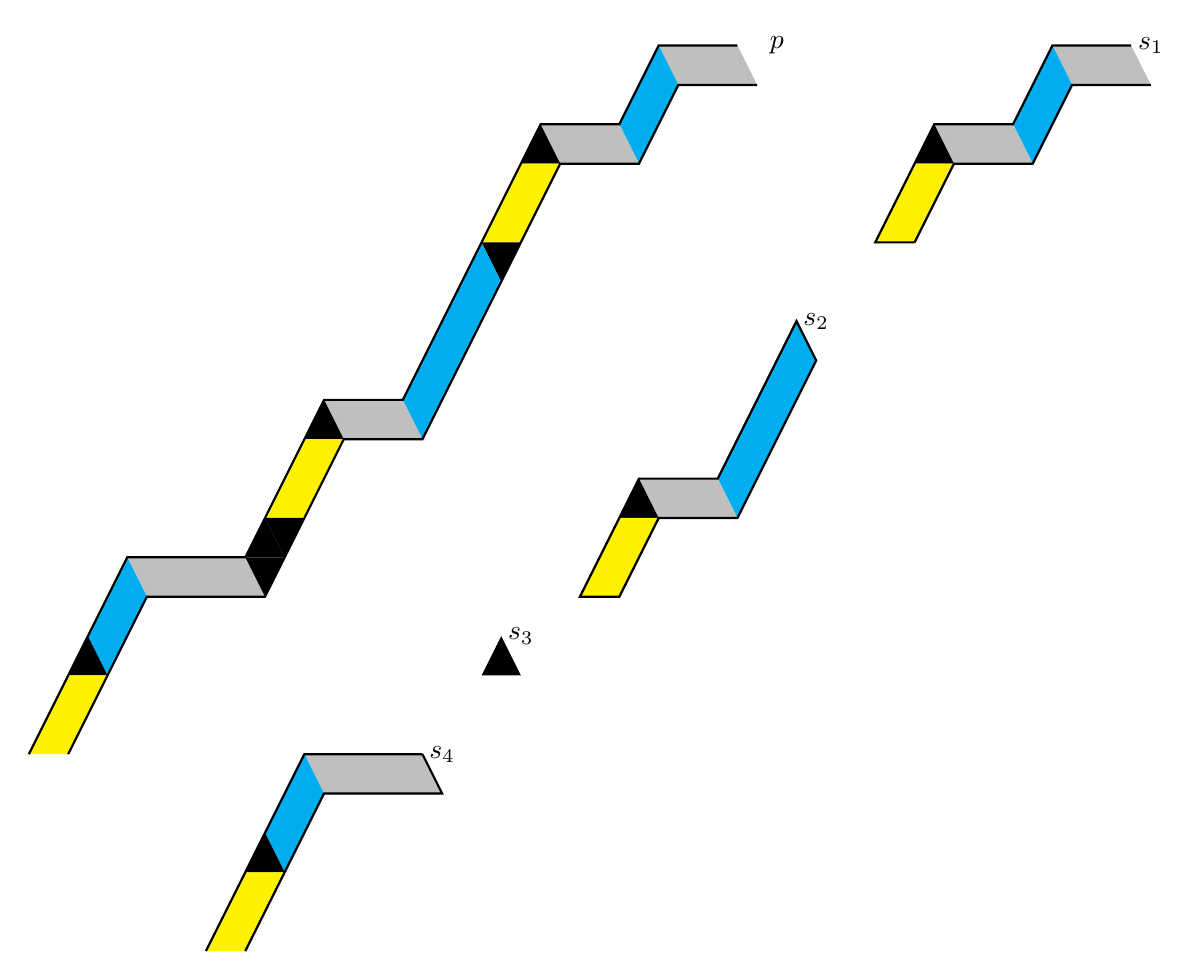
\begin{tikzpicture}


    \node at (8+16/4,16-14/2) {$p$};
    \fill[lightgray] (8+14/4,16-14/2)-- ++(-1,0)-- ++(1/4,-1/2)-- ++(1,0)--cycle;
    \fill[cyan] (8+10/4,16-14/2)-- ++(-1/2,-1)-- ++(1/4,-1/2)-- ++(1/2,1)--cycle;
    \fill[lightgray] (8+8/4,16-16/2)-- ++(-1,0)-- ++(1/4,-1/2)-- ++(1,0)--cycle;
    \fill[black] (8+4/4, 16-16/2)-- ++(-1/4,-1/2)-- ++(1/2,0)--cycle;
    \fill[yellow] (8+3/4, 16-17/2)-- ++(-1/2,-1)-- ++(1/2,0)-- ++(1/2,1)--cycle;
    \fill[black] (8+1/4,16-19/2)-- ++(1/2,0)-- ++(-1/4,-1/2)--cycle;
    \fill[cyan] (8+1/4,16-19/2)-- ++(-1,-2)-- ++(1/4,-1/2)-- ++(1,2)--cycle;
    \fill[lightgray] (8-3/4,16-23/2)-- ++(-1,0)-- ++(1/4,-1/2)-- ++(1,0)--cycle;
    \fill[black] (8-7/4,16-23/2)-- ++(-1/4,-1/2)-- ++(1/2,0)--cycle;
    \fill[yellow] (8-8/4,16-24/2)-- ++(-1/2,-1)-- ++(1/2,0)-- ++(1/2,1)--cycle;
    \fill[black] (8-10/4,16-26/2)-- ++(1/2,0)-- ++(-1/4,-1/2)--cycle;
    \fill[lightgray] (8-11/4,16-27/2)-- ++(-3/2,0)-- ++(1/4,-1/2)-- ++(3/2,0)--cycle;
    \fill[black] (8-10/4,16-26/2)-- ++(-1/4,-1/2)-- ++(1/2,0)--cycle;
    \fill[black] (8-9/4,16-27/2)-- ++(-1/2,0)-- ++(1/4,-1/2)--cycle;
    \fill[cyan] (8-17/4,16-27/2)-- ++(-2/4,-2/2)-- ++(1/4,-1/2)-- ++(2/4,2/2)--cycle;
    \fill[black] (8-19/4,16-29/2)-- ++(-1/4,-1/2)-- ++(1/2,0)--cycle;
    \fill[yellow] (8-20/4,16-30/2)-- ++(-1/2,-1)-- ++(1/2,0)-- ++(1/2,1)--cycle;


    \draw[thick] (8+14/4,16-14/2)-- ++(-1,0)-- ++(-1/2,-1)-- ++(-1,0)-- ++(-7/4,-7/2)-- ++(-1,0)-- ++(-4/4,-4/2)-- ++(-3/2,0)-- ++(-5/4,-5/2);
    \draw[thick] (8+15/4, 16-15/2)-- ++(-1,0)-- ++(-1/2,-1)-- ++(-1,0)-- ++(-7/4,-7/2)-- ++(-1,0)-- ++(-4/4,-4/2)-- ++(-3/2,0)-- ++(-4/4,-4/2);

    \begin{scope}[xshift=5cm]
    \node at (8+15/4,16-14/2) {$s_1$};
    \fill[lightgray] (8+14/4,16-14/2)-- ++(-1,0)-- ++(1/4,-1/2)-- ++(1,0)--cycle;
    \fill[cyan] (8+10/4,16-14/2)-- ++(-1/2,-1)-- ++(1/4,-1/2)-- ++(1/2,1)--cycle;
    \fill[lightgray] (8+8/4,16-16/2)-- ++(-1,0)-- ++(1/4,-1/2)-- ++(1,0)--cycle;
    \fill[black] (8+4/4, 16-16/2)-- ++(-1/4,-1/2)-- ++(1/2,0)--cycle;
    \fill[yellow] (8+3/4, 16-17/2)-- ++(-1/2,-1)-- ++(1/2,0)-- ++(1/2,1)--cycle;
    
    \draw[thick] (8+14/4,16-14/2)-- ++(-1,0)-- ++(-1/2,-1)-- ++(-1,0)-- ++(-3/4,-3/2)-- ++(1/2,0);
    \draw[thick] (8+15/4, 16-15/2)-- ++(-1,0)-- ++(-1/2,-1)-- ++(-1,0)-- ++(-2/4,-2/2);
    \end{scope}

    \begin{scope}[xshift=4cm, yshift=-1cm]
    \node at (8+2/4,16-19/2) {$s_2$};
    \fill[cyan] (8+1/4,16-19/2)-- ++(-1,-2)-- ++(1/4,-1/2)-- ++(1,2)--cycle;
    \fill[lightgray] (8-3/4,16-23/2)-- ++(-1,0)-- ++(1/4,-1/2)-- ++(1,0)--cycle;
    \fill[black] (8-7/4,16-23/2)-- ++(-1/4,-1/2)-- ++(1/2,0)--cycle;
    \fill[yellow] (8-8/4,16-24/2)-- ++(-1/2,-1)-- ++(1/2,0)-- ++(1/2,1)--cycle;

    \draw[thick] (8+1/4,16-19/2)-- ++(-1,-2)-- ++(-1,0)-- ++(-3/4,-3/2)-- ++(1/2,0)-- ++(2/4,2/2)-- ++(1,0)-- ++(1,2)--cycle;
    \end{scope}

    \begin{scope}[xshift=3cm, yshift=-1.5cm]
      \fill[black] (8-10/4,16-26/2)-- ++(-1/4,-1/2)-- ++(1/2,0)--cycle;
      \node at (8-9/4,16-26/2) {$s_3$};
    \end{scope}

    \begin{scope}[xshift=2cm, yshift=-3cm]
      \node at(8-9/4,16-26/2) {$s_4$};
      \fill[lightgray] (8-10/4,16-26/2)-- ++(-3/2,0)-- ++(1/4,-1/2)-- ++(3/2,0)--cycle;
    \fill[cyan] (8-16/4,16-26/2)-- ++(-2/4,-2/2)-- ++(1/4,-1/2)-- ++(2/4,2/2)--cycle;
    \fill[black] (8-18/4,16-28/2)-- ++(-1/4,-1/2)-- ++(1/2,0)--cycle;
    \fill[yellow] (8-19/4,16-29/2)-- ++(-1/2,-1)-- ++(1/2,0)-- ++(1/2,1)--cycle;

    \draw[thick] (8-10/4,16-26/2)-- ++(-3/2,0)-- ++(-5/4,-5/2);
    \draw[thick] (8-10/4,16-26/2)-- ++(1/4,-1/2)-- ++(-1.5,0)-- ++(-4/4,-4/2);
    \end{scope}
  \end{tikzpicture}

\end{document}
  \caption{path $p$とそのsegment $s_1,s_2,s_3,s_4$.$s_3$の長さは$0$である.}\label{path,segment}
\end{figure}

\newpage
puzzle $P$のpathを左側から順に$p_1,\cdots,p_t$とする.次の操作を行って得られるedge labeled tableauxを$\varphi(P)$とする.

$p_1$のsegmentを上から順に$s_1,\cdots,s_a$, $(a\leq k)$とする.$s_1$に

\begin{tikzpicture}[baseline=-1pt]
  \fill[cyan] (0,0)--(0.25,0.42)--(0.5,0)--(0.25,-0.42)--cycle;
  \draw[thick] (0,0)--(0.25,0.42)--(0.5,0)--(0.25,-0.42)--cycle;
\end{tikzpicture}
と

\begin{tikzpicture}[baseline=2pt]
  \fill[lightgray] (0,0)-- ++(0.5,0)-- ++(-0.25,0.42)-- ++(-0.5,0)--cycle;
  \draw[thick](0,0)-- ++(0.5,0)-- ++(-0.25,0.42)-- ++(-0.5,0)--cycle;
\end{tikzpicture}
がそれぞれ$a_1,a_2,\cdots,a_u$個,$b_1,b_2,\cdots,b_u$個交互に現れ,

\begin{tikzpicture}[baseline=2pt]
  \fill[yellow] (0,0)-- ++(0.5,0)-- ++(0.25,0.42)-- ++(-0.5,0)--cycle;
  \draw[thick](0,0)-- ++(0.5,0)-- ++(0.25,0.42)-- ++(-0.5,0)--cycle;
\end{tikzpicture}
が$c$個現れるとする.ただし$a_i,b_j,c\geq 0$であるとする.

$\Lambda=\overbrace{(n,\cdots,n)}^{k\text{-copies}}$の$k$行目に次のようにedge labelとbox labelを書き入れていく.まず左から$a_1$個のboxの下辺のedge labelに$1$から$a_1$を1つずつ,左から単調増大になるように入れる.次の右隣りの$b_1$個のboxには何もせず,次の$a_2$個のboxのedge labelに$a_1+1$から$a_1+a_2$を単調増大になるように入れていく.これを$b_u$まで行ったのち,$c$個のboxに$a_1+\cdots+a_u+1$から$a_1+\cdots+a_u+c$までを左から単調増大になるように入れる(図\ref{process for segment}).

\begin{figure}[H]
  \centering
  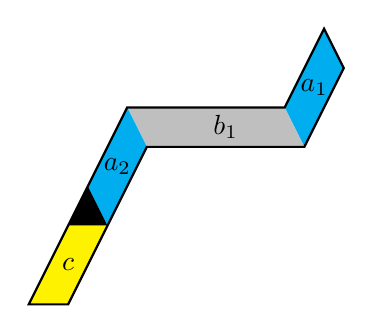
\begin{tikzpicture}
    \fill[cyan] (8+19/4,16-19/2)-- ++(-1/2,-1)-- ++(1/4,-1/2)-- ++(1/2,1)--cycle;
    \node at (8+18/4+1/8,16-20/2-1/4) {$a_1$};
    \fill[lightgray] (8+17/4,16-21/2)-- ++(-2,0)-- ++(1/4,-1/2)-- ++(2,0)--cycle;
    \node at (8+14/4,16-21/2-1/4) {$b_1$};
    \fill[cyan] (8+9/4,16-21/2)-- ++(-2/4,-2/2)-- ++(1/4,-1/2)-- ++(2/4,2/2)--cycle;
    \node at (8+8/4+1/8,16-22/2-1/4) {$a_2$};
    \fill[black] (8+7/4,16-23/2)-- ++(-1/4,-1/2)-- ++(1/2,0)--cycle;
    \fill[yellow] (8+6/4,16-24/2)-- ++(-2/4,-2/2)-- ++(1/2,0)-- ++(1/2,1)--cycle;
    \node at (8+5/4+2/8,16-25/2) {$c$};

    \draw[thick](8+19/4,16-19/2)-- ++(-2/4,-1)-- ++(-4/2,0)-- ++(-5/4,-5/2)-- ++(1/2,0)-- ++(4/4,4/2)-- ++(4/2,0)-- ++(2/4,2/2)--cycle;
  \end{tikzpicture}
  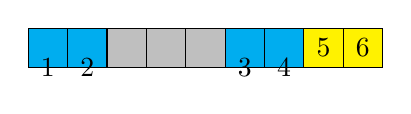
\begin{tikzpicture}
    \fill[cyan] (0,0) rectangle (1, 0.5);
      \fill[lightgray] (1,0) rectangle (2.5,0.5);
      \fill[cyan] (2.5,0) rectangle (3.5,0.5);
      \fill[yellow] (3.5,0) rectangle (4.5,0.5);
      \draw (0,0) rectangle (4.5, 0.5);
      \foreach \x in {1,...,8} {
        \draw (\x * 0.5, 0) -- ++(0, 0.5);
      }
  
      \node at (0.25,0) {$1$};
      \node at (0.75,0) {$2$};
      \node at (2.75,0) {$3$};
      \node at (3.25,0) {$4$};
      \node at (3.75,0.25) {$5$};
      \node at (4.25,0.25) {$6$};
  \end{tikzpicture}
  \caption{$a_1=2,b_1=3,a_2=2,c=2$の場合のsegmentに対する処理.}\label{process for segment}
\end{figure}

次のsegment $s_2$に対して,$\Lambda$の$k-1$行目のedge labelとbox labelを同様の方法で書き入れていく.ただし$k$行目で最後に処理を行ったboxのすぐ右上のboxから処理を始める.また$s_1$の長さが$0$であった場合は,$k-1$行目の最も左にある箱から処理を行う.同様にしてすべてのsegmentに対してedge labelとbox labelを書き入れていく.$s_i$の長さが$0$であったなら,$k-i+1$行の処理はスキップして,$s_{i+1}$に対する処理は,直前に処理を行ったboxのすぐ右の列にある$k-i$行目のboxから始める(図\ref{process for path}).


\begin{figure}[H]
  \centering
  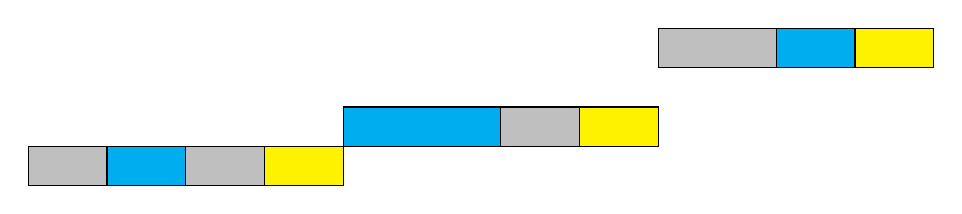
\begin{tikzpicture}
    \draw (0,0) rectangle (8 * 1/2, 1/2);
    \draw (8 * 1/2,1/2) rectangle (16 * 1/2, 1);
    \draw (16 * 1/2,3/2) rectangle (23 * 1/2, 2);

    \fill[lightgray] (0,0) rectangle (1,1/2);
    \draw (0,0) rectangle (1,1/2);
    \fill[cyan] (1,0) rectangle (2,1/2);
    \draw (1,0) rectangle (2,1/2);
    \fill[lightgray] (2,0) rectangle (3,1/2);
    \draw (2,0) rectangle (3,1/2);
    \fill[yellow] (3,0) rectangle ++(1,1/2);
    \draw (3,0) rectangle ++(1,1/2);
    
    \fill[cyan] (4,1/2) rectangle ++(4/2,1/2);
    \draw (4,1/2) rectangle ++(4/2,1/2);
    \fill[lightgray] (6,1/2) rectangle ++(1,1/2);
    \draw (6,1/2) rectangle ++(1,1/2);
    \fill[yellow] (7,1/2) rectangle ++(1,1/2);
    \draw (7,1/2) rectangle ++(1,1/2);

    \fill[lightgray] (8,3/2) rectangle ++(3/2,1/2);
    \draw (8,3/2) rectangle ++(3/2,1/2);
    \fill[cyan] (19/2,3/2) rectangle ++(1,1/2);
    \draw (19/2,3/2) rectangle ++(1,1/2);
    \fill[yellow] (21/2,3/2) rectangle ++(1,1/2);
    \draw (21/2,3/2) rectangle ++(1,1/2);
  \end{tikzpicture}
  \caption{
  図\ref{path,segment}のpathに対する処理.青い領域のboxの下辺にedge labelが入り,黄色い領域のboxにはbox labelが入っている.灰色の領域のboxには何も書かれていない.また,$s_3$の長さが$0$であるから,図のように下から$3$行目に対する処理をスキップする.}\label{process for path}
\end{figure}

次に$p_2$に対して同じ操作を行う.ただし$p_1$に対する操作で最後に書き入れたラベルを$l$とすると,$p_2$に対する操作で書き入れるlabelは$l+1$から始める.すべてのpathに対して同様の操作を行い,box labelの入った領域を含む左上の部分を$\varphi(P)$とする.作り方から$\varphi(P)$が定義\ref{label condition}にあるラベルに関する条件を満たすことは明らかである.

\begin{eg}
  図\ref{eg of varphi}のpuzzle $P$に対して$\varphi(P)$を計算する.
  \begin{figure}[H]
    \centering
    \documentclass{ltjsarticle}
\RequirePackage{luatex85}
\usepackage[utf8]{inputenc}
\usepackage[dvipdfmx]{color}
\usepackage{enumerate}
\usepackage{here}
\usepackage{amsthm}
\usepackage{amsfonts}
\usepackage{amsmath}
\usepackage{amssymb}
\usepackage{latexsym}
\usepackage{ytableau}
\usepackage{docmute}
\usepackage{mathtools}
\usepackage{xr}
\usepackage{tikz}
\usetikzlibrary{intersections, calc, arrows.meta}
\usepackage[all]{xy}
\usepackage{graphics}
\usepackage[luatex]{hyperref}
%\usepackage{pxjahyper}



\theoremstyle{definition}
\newtheorem{defin}{定義}[subsection]
\newtheorem{theo}[defin]{定理}
\newtheorem{cor}[defin]{系}
\newtheorem{prop}[defin]{命題}
\newtheorem{lemm}[defin]{補題}
\newtheorem{notice}[defin]{注意}
\newtheorem{eg}[defin]{例}
\newtheorem{fact}[defin]{事実}


\renewcommand{\labelenumi}{(\roman{enumi})}


\newcommand{\invlimit}{\mathop{\lim_{\longleftarrow}}}
\newcommand{\dirlimit}{\mathop{\lim_{\longrightarrow}}}
\newcommand{\ind}{\text{Ind}}
\newcommand{\Hom}{\text{Hom}}
\newcommand{\tr}{\text{tr}}
\newcommand{\id}[1]{\text{id}_{#1}}
\newcommand{\sgn}{\mathrm{sgn}}
\newcommand{\res}[1]{\text{Res}_{#1}}
\newcommand{\generated}[1]{\langle\:#1\:\rangle}
\newcommand{\im}{\text{Im }}
\newcommand{\rank}{\text{rank }}
\newcommand{\del}[2]{\frac{\partial #1}{\partial #2}}
\newcommand{\delsametwo}[2]{\frac{\partial^2 #1}{\partial #2^2}}
\newcommand{\delothertwo}[3]{\frac{\partial^2#1}{\partial#2\partial#3}}
\newcommand{\ddel}[2]{\frac{\partial}{\partial #2}#1}
\newcommand{\ddelsametwo}[3]{\frac{\partial^2}{\partial #2^2}#1}
\newcommand{\ddelothertwo}[3]{\frac{\partial^2}{\partial#2\partial#3}#1}
\newcommand{\simneq}{\not\simeq}
\newcommand{\transpose}[1]{^t\!#1}
\newcommand{\ie}{\text{i.e.}}
\newcommand{\inv}[1]{#1^{-1}}
\newcommand{\real}{\mathbb{R}}
\newcommand{\complex}{\mathbb{C}}
\newcommand{\integer}{\mathbb{Z}}
\newcommand{\quotient}{\mathbb{Q}}
\newcommand{\natnum}{\mathbb{N}}
\newcommand{\proj}{\mathbb{P}}
\newcommand{\affine}{\mathbb{A}}
\newcommand{\tensor}[3]{#1\otimes_#2#3}
\newcommand{\map}[3]{#1:#2\rightarrow#3}
\newcommand{\aut}[2]{\mathrm{Aut}_{#1} (#2)}
\newcommand{\hommoph}[2]{\mathrm{Hom}_{#1}(#2)}
\newcommand{\gl}{\text{GL}}
\newcommand{\End}{\text{End}}
\newcommand{\set}[2]{\left\{\:#1\:\middle|\:#2\:\right\}}
\newcommand{\pmat}[1]{\begin{pmatrix} #1
\end{pmatrix}}
\newcommand{\vmat}[1]{\begin{vmatrix} #1
\end{vmatrix}}
\newcommand{\bmat}[1]{\begin{bmatrix} #1
\end{bmatrix}}
\newcommand{\br}{\vskip\baselineskip}
\newcommand{\Lie}{\text{Lie}}
\newcommand{\Sym}{\text{Sym}}
\newcommand{\Alt}{\text{Alt}}
\newcommand{\ch}{\text{ch}}
\newcommand{\diag}{\text{diag}}
\newcommand{\comb}[2]{_{#1}C_{#2}}
\newcommand{\codim}{\text{codim}\:}
\newcommand{\yd}[1]{\ydiagram{#1}}

\title{aaa}
\author{}
\date{}


\begin{document}
\maketitle

  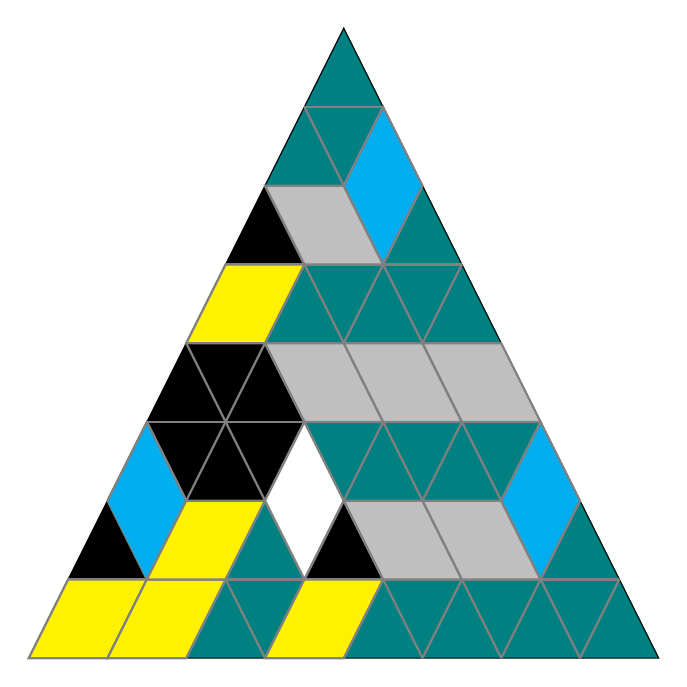
\begin{tikzpicture}
    \fill[teal] (0,0)-- ++(8,0)-- ++(-4,8)--cycle;
    \draw (0,0)-- ++(8,0)-- ++(-4,8)--cycle;

    \fill[black] (2,2)--++(1,0)--++(1/2,1)-- ++(-1/2,1)--++(-1,0)-- ++(-1/2,-1)-- ++(-1/2,-1);
    \fill[black] (1/2,1)-- ++(1,0)-- ++(-1/2,1)--cycle;
    \fill[black] (2.5, 5)-- ++(1,0)-- ++(-1/2,1)--cycle;
    \fill[black] (4,2)-- ++(1/2,-1)-- ++(-1,0)--cycle;

    \foreach \x in {1,...,7}{
      \draw[gray,thick] (\x, 0) -- (\x/2, \x);
      \draw[gray,thick] (\x, 0) -- (4+\x/2, 8-\x);
      \draw[gray,thick] (\x/2,\x) -- (8-\x/2,\x);
    };
    
    \fill[yellow] (0,0)-- ++(1,0)-- ++(1/2,1)--++(-1,0)--cycle;
    \draw[gray,thick](0,0)-- ++(1,0)-- ++(1/2,1)--++(-1,0)--cycle;
    \fill[cyan] (3/2,1)-- ++(1/2,1)-- ++(-1/2,1)-- ++(-1/2,-1);
    \draw[gray,thick](3/2,1)-- ++(1/2,1)-- ++(-1/2,1)-- ++(-1/2,-1);
    \fill[yellow] (2,4)-- ++(1,0)-- ++(1/2,1)-- ++(-1,0)--cycle;
    \draw[gray,thick](2,4)-- ++(1,0)-- ++(1/2,1)-- ++(-1,0)--cycle;
    \fill[lightgray] (3,6)-- ++(1,0)-- ++(1/2,-1)-- ++(-1,0)--cycle;
    \draw[gray,thick](3,6)-- ++(1,0)-- ++(1/2,-1)-- ++(-1,0)--cycle;
    \fill[cyan] (4,6)-- ++(1/2,-1)-- ++(1/2,1)-- ++(-1/2,1)--cycle;
    \draw[gray,thick](4,6)-- ++(1/2,-1)-- ++(1/2,1)-- ++(-1/2,1)--cycle;
    \fill[yellow] (1,0)-- ++(1,0)-- ++(1/2,1)--++(-1,0)--cycle;
    \draw[gray,thick](1,0)-- ++(1,0)-- ++(1/2,1)--++(-1,0)--cycle;
    \fill[yellow] (3/2,1)-- ++(1,0)-- ++(1/2,1)--++(-1,0)--cycle;
    \draw[gray,thick](3/2,1)-- ++(1,0)-- ++(1/2,1)--++(-1,0)--cycle;

    \fill[lightgray](3,4)-- ++(1,0)-- ++(1/2,-1)-- ++(-1,0)--cycle;
    \draw[gray,thick](3,4)-- ++(1,0)-- ++(1/2,-1)-- ++(-1,0)--cycle;

    \fill[lightgray](4,4)-- ++(1,0)-- ++(1/2,-1)-- ++(-1,0)--cycle;
    \draw[gray,thick](4,4)-- ++(1,0)-- ++(1/2,-1)-- ++(-1,0)--cycle;

    \fill[lightgray](5,4)-- ++(1,0)-- ++(1/2,-1)-- ++(-1,0)--cycle;
    \draw[gray,thick](5,4)-- ++(1,0)-- ++(1/2,-1)-- ++(-1,0)--cycle;

    \fill[white] (3,2)-- ++(1/2,1)-- ++(1/2,-1)-- ++(-1/2,-1)--cycle;
    \draw[gray,thick](3,2)-- ++(1/2,1)-- ++(1/2,-1)-- ++(-1/2,-1)--cycle;

    \fill[yellow] (3,0)-- ++(1,0)-- ++(1/2,1)--++(-1,0)--cycle;
    \draw[thick,gray] (3,0)-- ++(1,0)-- ++(1/2,1)--++(-1,0)--cycle;

    \fill[lightgray] (4,2)-- ++(1,0)-- ++(1/2,-1)-- ++(-1,0)--cycle;
    \draw[gray, thick] (4,2)-- ++(1,0)-- ++(1/2,-1)-- ++(-1,0)--cycle;

    \fill[lightgray] (5,2)-- ++(1,0)-- ++(1/2,-1)-- ++(-1,0)--cycle;
    \draw[gray, thick] (5,2)-- ++(1,0)-- ++(1/2,-1)-- ++(-1,0)--cycle;

    \fill[cyan] (6,2)-- ++(1/2,-1)-- ++(1/2,1)-- ++(-1/2,1)--cycle;
    \draw[gray,thick] (6,2)-- ++(1/2,-1)-- ++(1/2,1)-- ++(-1/2,1)--cycle;
  \end{tikzpicture}

\end{document}
    \caption{puzzle $P\in\mathcal{P}^{11010000}_{01010100,01001100}$}\label{eg of varphi}
  \end{figure}
  $P$のpathは図$\ref{paths of P}$の$p_1,p_2,p_3$の3つである.
  \documentclass{ltjsarticle}
\RequirePackage{luatex85}
\usepackage[utf8]{inputenc}
\usepackage[dvipdfmx]{color}
\usepackage{enumerate}
\usepackage{here}
\usepackage{amsthm}
\usepackage{amsfonts}
\usepackage{amsmath}
\usepackage{amssymb}
\usepackage{latexsym}
\usepackage{ytableau}
\usepackage{docmute}
\usepackage{mathtools}
\usepackage{xr}
\usepackage{tikz}
\usetikzlibrary{intersections, calc, arrows.meta}
\usepackage[all]{xy}
\usepackage{graphics}
\usepackage[luatex]{hyperref}
%\usepackage{pxjahyper}



\theoremstyle{definition}
\newtheorem{defin}{定義}[subsection]
\newtheorem{theo}[defin]{定理}
\newtheorem{cor}[defin]{系}
\newtheorem{prop}[defin]{命題}
\newtheorem{lemm}[defin]{補題}
\newtheorem{notice}[defin]{注意}
\newtheorem{eg}[defin]{例}
\newtheorem{fact}[defin]{事実}


\renewcommand{\labelenumi}{(\roman{enumi})}


\newcommand{\invlimit}{\mathop{\lim_{\longleftarrow}}}
\newcommand{\dirlimit}{\mathop{\lim_{\longrightarrow}}}
\newcommand{\ind}{\text{Ind}}
\newcommand{\Hom}{\text{Hom}}
\newcommand{\tr}{\text{tr}}
\newcommand{\id}[1]{\text{id}_{#1}}
\newcommand{\sgn}{\mathrm{sgn}}
\newcommand{\res}[1]{\text{Res}_{#1}}
\newcommand{\generated}[1]{\langle\:#1\:\rangle}
\newcommand{\im}{\text{Im }}
\newcommand{\rank}{\text{rank }}
\newcommand{\del}[2]{\frac{\partial #1}{\partial #2}}
\newcommand{\delsametwo}[2]{\frac{\partial^2 #1}{\partial #2^2}}
\newcommand{\delothertwo}[3]{\frac{\partial^2#1}{\partial#2\partial#3}}
\newcommand{\ddel}[2]{\frac{\partial}{\partial #2}#1}
\newcommand{\ddelsametwo}[3]{\frac{\partial^2}{\partial #2^2}#1}
\newcommand{\ddelothertwo}[3]{\frac{\partial^2}{\partial#2\partial#3}#1}
\newcommand{\simneq}{\not\simeq}
\newcommand{\transpose}[1]{^t\!#1}
\newcommand{\ie}{\text{i.e.}}
\newcommand{\inv}[1]{#1^{-1}}
\newcommand{\real}{\mathbb{R}}
\newcommand{\complex}{\mathbb{C}}
\newcommand{\integer}{\mathbb{Z}}
\newcommand{\quotient}{\mathbb{Q}}
\newcommand{\natnum}{\mathbb{N}}
\newcommand{\proj}{\mathbb{P}}
\newcommand{\affine}{\mathbb{A}}
\newcommand{\tensor}[3]{#1\otimes_#2#3}
\newcommand{\map}[3]{#1:#2\rightarrow#3}
\newcommand{\aut}[2]{\mathrm{Aut}_{#1} (#2)}
\newcommand{\hommoph}[2]{\mathrm{Hom}_{#1}(#2)}
\newcommand{\gl}{\text{GL}}
\newcommand{\End}{\text{End}}
\newcommand{\set}[2]{\left\{\:#1\:\middle|\:#2\:\right\}}
\newcommand{\pmat}[1]{\begin{pmatrix} #1
\end{pmatrix}}
\newcommand{\vmat}[1]{\begin{vmatrix} #1
\end{vmatrix}}
\newcommand{\bmat}[1]{\begin{bmatrix} #1
\end{bmatrix}}
\newcommand{\br}{\vskip\baselineskip}
\newcommand{\Lie}{\text{Lie}}
\newcommand{\Sym}{\text{Sym}}
\newcommand{\Alt}{\text{Alt}}
\newcommand{\ch}{\text{ch}}
\newcommand{\diag}{\text{diag}}
\newcommand{\comb}[2]{_{#1}C_{#2}}
\newcommand{\codim}{\text{codim}\:}
\newcommand{\yd}[1]{\ydiagram{#1}}

\title{aaa}
\author{}
\date{}


\begin{document}
\maketitle

\begin{figure}[H]
  \centering
  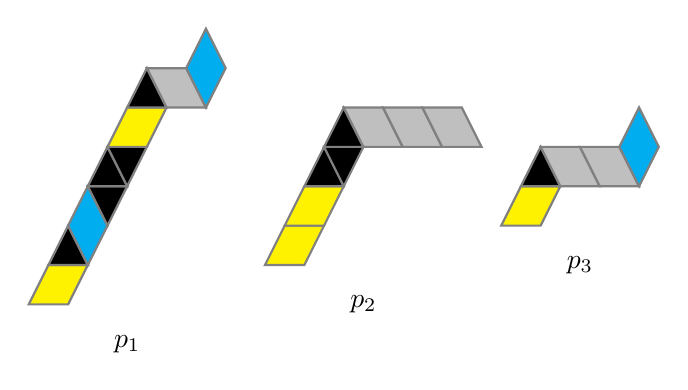
\begin{tikzpicture}
    \begin{scope}
      \node at (5/4, -1/2) {$p_1$};
      \fill[yellow] (0,0)-- ++(1/2,0)-- ++(1/4,1/2)-- ++(-1/2,0)--cycle;
      \draw[thick,gray] (0,0)-- ++(1/2,0)-- ++(1/4,1/2)-- ++(-1/2,0)--cycle;

      \filldraw[fill=black, draw=gray,thick] (1/4,1/2)-- ++(1/2,0)-- ++(-1/4,1/2)--cycle;

      \filldraw[fill=cyan, draw=gray,thick] (1/2,1)-- ++(1/4,-1/2)-- ++(1/4,1/2)-- ++(-1/4,1/2)--cycle;

      \fill[black] (1,1)-- ++(1/4,1/2)-- ++(-1/2,0)--cycle;
      \draw[thick,gray] (1,1)-- ++(1/4,1/2)-- ++(-1/2,0)--cycle;

      \fill[black] (3/4,1+1/2)-- ++(1/2,0)-- ++(-1/4,1/2)--cycle;
      \draw[thick,gray] (3/4,1+1/2)-- ++(1/2,0)-- ++(-1/4,1/2)--cycle;

      \fill[black] (1+1/4,1+1/2)-- ++(1/4,1/2)-- ++(-1/2,0)--cycle;
      \draw[thick,gray] (1+1/4,1+1/2)-- ++(1/4,1/2)-- ++(-1/2,0)--cycle;

      \filldraw[fill=yellow, draw=gray,thick] (1,2)-- ++(1/2,0)-- ++(1/4,1/2)-- ++(-1/2,0)--cycle;

      \filldraw[fill=black, draw=gray,thick] (5/4,5/2)-- ++(1/2,0)-- ++(-1/4,1/2)--cycle;

      \filldraw[fill=lightgray, draw=gray,thick] (6/4,6/2)-- ++(1/2,0)-- ++(1/4,-1/2)-- ++(-1/2,0)--cycle;

      \filldraw[fill=cyan, draw=gray,thick] (8/4,6/2)-- ++(1/4,-1/2)-- ++(1/4,1/2)-- ++(-1/4,1/2)--cycle;
    \end{scope}
    \begin{scope}[xshift=3cm, yshift=0.5cm]
      \node at (5/4, -1/2) {$p_2$};
      \filldraw[fill=yellow, draw=gray,thick] (0,0)-- ++(1/2,0)-- ++(1/4,1/2)-- ++(-1/2,0)--cycle;
      \filldraw[fill=yellow, draw=gray,thick] (1/4,1/2)-- ++(1/2,0)-- ++(1/4,1/2)-- ++(-1/2,0)--cycle;
      \filldraw[fill=black, draw=gray,thick] (1/2,1)-- ++(1/2,0)-- ++(-1/4,1/2)--cycle;
      %
      \filldraw[fill=black, draw=gray,thick] (3/4,3/2)-- ++(1/2,0)-- ++(-1/4,-1/2)--cycle;
      \filldraw[fill=black, draw=gray,thick] (3/4,3/2)-- ++(1/2,0)-- ++(-1/4,1/2)--cycle;
      \filldraw[fill=lightgray, draw=gray,thick] (4/4,4/2)-- ++(1/2,0)-- ++(1/4,-1/2)-- ++(-1/2,0)--cycle;
      \filldraw[fill=lightgray, draw=gray,thick] (6/4,4/2)-- ++(1/2,0)-- ++(1/4,-1/2)-- ++(-1/2,0)--cycle;
      \filldraw[fill=lightgray, draw=gray,thick] (8/4,4/2)-- ++(1/2,0)-- ++(1/4,-1/2)-- ++(-1/2,0)--cycle;
    \end{scope}
    \begin{scope}[xshift=6cm, yshift=1cm]
      \node at (4/4, -1/2) {$p_3$};
      \filldraw[fill=yellow, draw=gray,thick] (0,0)-- ++(1/2,0)-- ++(1/4,1/2)-- ++(-1/2,0)--cycle;
      \filldraw[fill=black, draw=gray,thick] (1/4,1/2)-- ++(1/2,0)-- ++(-1/4,1/2)--cycle;
      \filldraw[fill=lightgray, draw=gray,thick] (2/4,2/2)-- ++(1/2,0)-- ++(1/4,-1/2)-- ++(-1/2,0)--cycle;
      \filldraw[fill=lightgray, draw=gray,thick] (4/4,2/2)-- ++(1/2,0)-- ++(1/4,-1/2)-- ++(-1/2,0)--cycle;
      \filldraw[fill=cyan, draw=gray,thick] (6/4,2/2)-- ++(1/4,-1/2)-- ++(1/4,1/2)-- ++(-1/4,1/2)--cycle;
    \end{scope}
  \end{tikzpicture}
  \caption{$P$のpath $p_1,p_2,p_3$.}\label{paths of P}
\end{figure}

\end{document}
  $p_1,p_2,p_3$に対して操作を行う(図\ref{eg of process})と$\varphi(P)\in \text{EqSYT}((5,5,4)/(4,3,2), 8)$であることがわかる(図\ref{varphi P}).
  \begin{figure}[H]
    \centering
    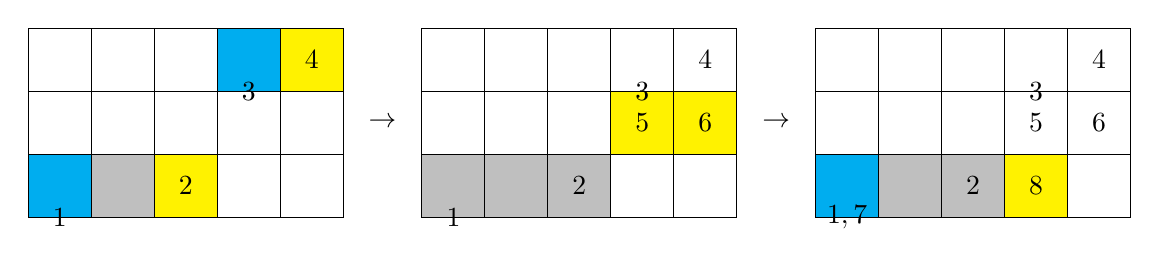
\begin{tikzpicture}
      \begin{scope}
        \fill[cyan] (0,0) rectangle ++(0.8,0.8);
        \fill[lightgray] (0.8,0) rectangle ++(0.8,0.8);
        \fill[yellow] (1.6,0) rectangle ++(0.8,0.8);

        \fill[cyan] (2.4,1.6) rectangle ++(0.8,0.8);
        \fill[yellow] (3.2,1.6) rectangle ++(0.8,0.8);

        \draw (0,0) rectangle (4, 2.4);
        \foreach \x in {1,...,4} {
          \draw (\x * 0.8, 0) -- (\x * 0.8, 2.4);
        };
        \foreach \x in {1,2} {
          \draw (0, \x * 0.8) -- (4, \x * 0.8);
        };

        \node at (0.4,0) {$1$};
        \node at (2, 0.4) {$2$};
        \node at (2.8, 1.6) {$3$};
        \node at (3.6, 2) {$4$};
        
        \node at (4.5, 1.2) {$\rightarrow$};
      \end{scope}
      \begin{scope}[xshift=5cm]
        \fill[lightgray] (0,0) rectangle ++(0.8,0.8);
        \fill[lightgray] (0.8,0) rectangle ++(0.8,0.8);
        \fill[lightgray] (1.6,0) rectangle ++(0.8,0.8);

        \fill[yellow] (2.4,0.8) rectangle ++(0.8,0.8);
        \fill[yellow] (3.2,0.8) rectangle ++(0.8,0.8);

        \draw (0,0) rectangle (4, 2.4);
        \foreach \x in {1,...,4} {
          \draw (\x * 0.8, 0) -- (\x * 0.8, 2.4);
        };
        \foreach \x in {1,2} {
          \draw (0, \x * 0.8) -- (4, \x * 0.8);
        };

        \node at (0.4,0) {$1$};
        \node at (2, 0.4) {$2$};
        \node at (2.8, 1.6) {$3$};
        \node at (3.6, 2) {$4$};
        \node at (2.8,1.2) {$5$};
        \node at (3.6,1.2) {$6$};

        \node at (4.5, 1.2) {$\rightarrow$};
      \end{scope}
      \begin{scope}[xshift=10cm]
        \fill[cyan] (0,0) rectangle ++(0.8,0.8);
        \fill[lightgray] (0.8,0) rectangle ++(0.8,0.8);
        \fill[lightgray] (1.6,0) rectangle ++(0.8,0.8);
        \fill[yellow] (2.4,0) rectangle ++(0.8,0.8);

        \draw (0,0) rectangle (4, 2.4);
        \foreach \x in {1,...,4} {
          \draw (\x * 0.8, 0) -- (\x * 0.8, 2.4);
        };
        \foreach \x in {1,2} {
          \draw (0, \x * 0.8) -- (4, \x * 0.8);
        };

        \node at (0.4,0) {$1,7$};
        \node at (2, 0.4) {$2$};
        \node at (2.8, 1.6) {$3$};
        \node at (3.6, 2) {$4$};
        \node at (2.8,1.2) {$5$};
        \node at (3.6,1.2) {$6$};
        \node at (2.8,0.4) {$8$};
      \end{scope}
    \end{tikzpicture}
    \caption{左から順に$p_1,p_2,p_3$に対して操作を行った結果.}\label{eg of process}
  \end{figure}
  \begin{figure}[H]
    \centering
    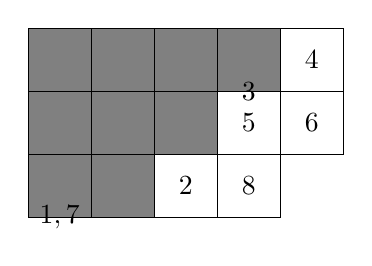
\begin{tikzpicture}
      \fill[gray] (0,0)-- ++(3.2,0)-- ++(0,-0.8)-- ++(-0.8,0)-- ++(0,-0.8)-- ++(-0.8,0)-- ++(0,-0.8)-- ++(-1.6,0)--cycle;
      \draw (0,0)-- ++(4,0)-- ++(0,-1.6)-- ++(-0.8,0)-- ++(0,-0.8)-- ++(-3.2,0)--cycle;
      \draw (0.8,0) -- ++(0,-2.4);
      \draw (1.6,0) -- ++(0,-2.4);
      \draw (2.4,0) -- ++(0,-2.4);
      \draw (3.2,0) -- ++(0,-2.4);
      \draw (0,-0.8) -- ++(4,0);
      \draw (0,-1.6) -- ++(4,0);

      \node at (0.4,-2.4) {$1,7$};
        \node at (2, -2) {$2$};
        \node at (2.8, -0.8) {$3$};
        \node at (3.6, -0.4) {$4$};
        \node at (2.8,-1.2) {$5$};
        \node at (3.6,-1.2) {$6$};
        \node at (2.8,-2) {$8$};
    \end{tikzpicture}
    \caption{$\varphi(P)\in\text{EqSYT}((5,5,4)/(4,3,2), 8)$}\label{varphi P}
  \end{figure}
\end{eg}

\begin{prop}
  $\lambda,\mu,\nu\in\binom{n}{k}$とする.
  $P\in\mathcal{P}^\nu_{\lambda\mu}$に対して$\varphi(P)\in\text{EqSYT}(\nu/\lambda,|\mu|)$である.
\end{prop}

\begin{proof}
  文字列$\lambda$は左から読んで$i_1,\cdots,i_k$番目に$1$が現れるとする.このとき
  \begin{align*}
    &l_j = i_{j+1} - i_{j} - 1,\quad (j=1,\cdots,k-1)\\
    &l_k = n - i_k
  \end{align*}
  とおく.同様に$\mu$に対しても$m_1,\cdots,m_{k}$,$\nu$に対しても$n_1,\cdots,n_{k}$を定義する.

  puzzle $P\in\mathcal{P}^\nu_{\lambda\mu}$のpathを左から順に$p_1,\cdots,p_k$,$p_i$のsegmentを上から順に$s_{i1},\cdots,s_{i,k-i+1}$,さらに$s_{ij}$の
  
\begin{tikzpicture}[baseline=2pt]
    \fill[yellow] (0,0)-- ++(0.5,0)-- ++(0.25,0.42)-- ++(-0.5,0)--cycle;
    \protect\draw[thick](0,0)-- ++(0.5,0)-- ++(0.25,0.42)-- ++(-0.5,0)--cycle;
  \end{tikzpicture}
  の部分を$s_{ij}^{\text{y}}$,
  
\begin{tikzpicture}[baseline=-1pt]
    \fill[cyan] (0,0)--(0.25,0.42)--(0.5,0)--(0.25,-0.42)--cycle;
    \protect\draw[thick] (0,0)--(0.25,0.42)--(0.5,0)--(0.25,-0.42)--cycle;
  \end{tikzpicture}
  ,
  
\begin{tikzpicture}[baseline=2pt]
    \fill[lightgray] (0,0)-- ++(0.5,0)-- ++(-0.25,0.42)-- ++(-0.5,0)--cycle;
    \protect\draw[thick](0,0)-- ++(0.5,0)-- ++(-0.25,0.42)-- ++(-0.5,0)--cycle;
  \end{tikzpicture}
  の部分を$s_{i,j}^{\text{bg}}$とおく.
  このとき
  \begin{align}
    &|s_{i,j}| = |s_{i+1,j}^{\text{bg}}| + |s_{i+1,j-1}^{\text{y}}| \quad \text{if } 1 < j < k-i+1\label{segment condition 1}\\
    &|s_{i,1}| = |s_{i+1,1}^{\text{bg}}|\label{segment condition 2}\quad \text{if } i < k\\
    &|s_{i,k-i+1}| = n_i + |s_{i+1, k-i}^{\text{y}}| \quad \text{if } i < k\label{segment condition 3}\\
    &|s_{k,1}| = n_k\label{segment condition 4}\\
    &|s_{1,i}^{\text{bg}}| + |s_{1,i-1}^{\text{y}}| = l_{k-i+1}\quad \text{if } i > 1\label{segment condition 5}\\
    &|s_{1,1}^{\text{bg}}| = l_{k}\label{segment condition 6}
  \end{align}
  である(図\ref{generic puzzle}).

  式(\ref{segment condition 1}),(\ref{segment condition 2})より$\varphi(P)$は図\ref{varphi of generic puzzle}のような形をしている.
  \documentclass{ltjsarticle}
\RequirePackage{luatex85}
\usepackage[utf8]{inputenc}
\usepackage[dvipdfmx]{color}
\usepackage{enumerate}
\usepackage{here}
\usepackage{amsthm}
\usepackage{amsfonts}
\usepackage{amsmath}
\usepackage{amssymb}
\usepackage{latexsym}
\usepackage{ytableau}
\usepackage{docmute}
\usepackage{mathtools}
\usepackage{xr}
\usepackage{tikz}
\usetikzlibrary{intersections, calc, arrows.meta}
\usepackage[all]{xy}
\usepackage{graphics}
\usepackage[luatex]{hyperref}
%\usepackage{pxjahyper}



\theoremstyle{definition}
\newtheorem{defin}{定義}[subsection]
\newtheorem{theo}[defin]{定理}
\newtheorem{cor}[defin]{系}
\newtheorem{prop}[defin]{命題}
\newtheorem{lemm}[defin]{補題}
\newtheorem{notice}[defin]{注意}
\newtheorem{eg}[defin]{例}
\newtheorem{fact}[defin]{事実}


\renewcommand{\labelenumi}{(\roman{enumi})}


\newcommand{\invlimit}{\mathop{\lim_{\longleftarrow}}}
\newcommand{\dirlimit}{\mathop{\lim_{\longrightarrow}}}
\newcommand{\ind}{\text{Ind}}
\newcommand{\Hom}{\text{Hom}}
\newcommand{\tr}{\text{tr}}
\newcommand{\id}[1]{\text{id}_{#1}}
\newcommand{\sgn}{\mathrm{sgn}}
\newcommand{\res}[1]{\text{Res}_{#1}}
\newcommand{\generated}[1]{\langle\:#1\:\rangle}
\newcommand{\im}{\text{Im }}
\newcommand{\rank}{\text{rank }}
\newcommand{\del}[2]{\frac{\partial #1}{\partial #2}}
\newcommand{\delsametwo}[2]{\frac{\partial^2 #1}{\partial #2^2}}
\newcommand{\delothertwo}[3]{\frac{\partial^2#1}{\partial#2\partial#3}}
\newcommand{\ddel}[2]{\frac{\partial}{\partial #2}#1}
\newcommand{\ddelsametwo}[3]{\frac{\partial^2}{\partial #2^2}#1}
\newcommand{\ddelothertwo}[3]{\frac{\partial^2}{\partial#2\partial#3}#1}
\newcommand{\simneq}{\not\simeq}
\newcommand{\transpose}[1]{^t\!#1}
\newcommand{\ie}{\text{i.e.}}
\newcommand{\inv}[1]{#1^{-1}}
\newcommand{\real}{\mathbb{R}}
\newcommand{\complex}{\mathbb{C}}
\newcommand{\integer}{\mathbb{Z}}
\newcommand{\quotient}{\mathbb{Q}}
\newcommand{\natnum}{\mathbb{N}}
\newcommand{\proj}{\mathbb{P}}
\newcommand{\affine}{\mathbb{A}}
\newcommand{\tensor}[3]{#1\otimes_#2#3}
\newcommand{\map}[3]{#1:#2\rightarrow#3}
\newcommand{\aut}[2]{\mathrm{Aut}_{#1} (#2)}
\newcommand{\hommoph}[2]{\mathrm{Hom}_{#1}(#2)}
\newcommand{\gl}{\text{GL}}
\newcommand{\End}{\text{End}}
\newcommand{\set}[2]{\left\{\:#1\:\middle|\:#2\:\right\}}
\newcommand{\pmat}[1]{\begin{pmatrix} #1
\end{pmatrix}}
\newcommand{\vmat}[1]{\begin{vmatrix} #1
\end{vmatrix}}
\newcommand{\bmat}[1]{\begin{bmatrix} #1
\end{bmatrix}}
\newcommand{\br}{\vskip\baselineskip}
\newcommand{\Lie}{\text{Lie}}
\newcommand{\Sym}{\text{Sym}}
\newcommand{\Alt}{\text{Alt}}
\newcommand{\ch}{\text{ch}}
\newcommand{\diag}{\text{diag}}
\newcommand{\comb}[2]{_{#1}C_{#2}}
\newcommand{\codim}{\text{codim}\:}
\newcommand{\yd}[1]{\ydiagram{#1}}

\title{aaa}
\author{}
\date{}


\begin{document}
\maketitle

\begin{figure}[H]
  \centering
  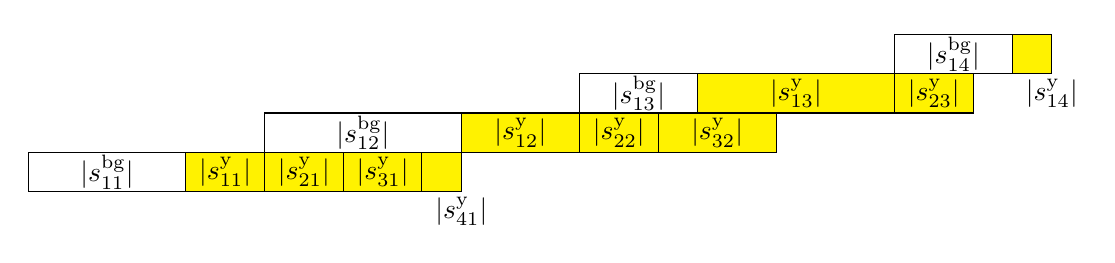
\begin{tikzpicture}
    \draw (0,0) rectangle ++(2,1/2);
    \node at (1,1/4) {$|s_{11}^{\text{bg}}|$};
    \filldraw[fill=yellow] (2,0) rectangle ++(1,1/2);
    \node at (2.5,1/4) {$|s_{11}^{\text{y}}|$};
    \filldraw[fill=yellow] (3,0) rectangle ++(1,1/2);
    \node at (3.5,1/4) {$|s_{21}^{\text{y}}|$};
    \filldraw[fill=yellow] (4,0) rectangle ++(1,1/2);
    \node at (4.5,1/4) {$|s_{31}^{\text{y}}|$};
    \filldraw[fill=yellow] (5,0) rectangle ++(1/2,1/2);
    \node at (5.5,-0.25) {$|s_{41}^{\text{y}}|$};

    \draw (3,1/2) rectangle ++(5/2,1/2);
    \node at (8/2+1/4,3/4) {$|s_{12}^{\text{bg}}|$};
    \filldraw[fill=yellow] (11/2, 1/2) rectangle ++(3/2,1/2);
    \node at (12/2+1/4,3/4) {$|s_{12}^{\text{y}}|$};
    \filldraw[fill=yellow] (14/2, 1/2) rectangle ++(2/2,1/2);
    \node at (15/2,3/4) {$|s_{22}^{\text{y}}|$};
    \filldraw[fill=yellow] (16/2, 1/2) rectangle ++(3/2,1/2);
    \node at (17/2+1/4,3/4) {$|s_{32}^{\text{y}}|$};

    \draw (14/2,1) rectangle ++(3/2,1/2);
    \node at (15/2 + 1/4,5/4) {$|s_{13}^{\text{bg}}|$};
    \filldraw[fill=yellow] (17/2,1) rectangle ++(5/2,1/2);
    \node at (19/2 + 1/4, 5/4) {$|s_{13}^{\text{y}}|$};
    \filldraw[fill=yellow] (22/2,1) rectangle ++(2/2,1/2);
    \node at (23/2, 5/4) {$|s_{23}^{\text{y}}|$};

    \draw (22/2,3/2) rectangle ++(3/2,1/2);
    \node at (23/2 + 1/4, 7/4) {$|s_{14}^{\text{bg}}|$};
    \filldraw[fill=yellow] (25/2,3/2) rectangle ++(1/2,1/2);
    \node at (26/2, 5/4) {$|s_{14}^{\text{y}}|$};
  \end{tikzpicture}
  \caption{図\ref{generic puzzle}のpuzzle $P$に対する$\varphi(P)$.黄色のboxにはbox labelが入っており,白いboxにはbox labelは入っていない.}\label{varphi of generic puzzle}
\end{figure}

\end{document}

  $\varphi(P)$の形が$\nu/\lambda$であることを示す.$\varphi(P)$のbox labelが入った領域の$k$行目の長さを計算すると

  \begin{align*}
    |s_{11}^{\text{bg}}| + |s_{11}^{\text{y}}| + |s_{21}^{\text{y}}| + \cdots + |s_{k,1}^{\text{y}}|
    &=|s_{11}| + |s_{21}^{\text{y}}| + \cdots + |s_{k,1}^{\text{y}}|\\
    &=|s_{21}^{\text{bg}}| + |s_{21}^{\text{y}}| + \cdots + |s_{k,1}^{\text{y}}|\\
    &=|s_{21}| + |s_{31}^{\text{y}}| + \cdots + |s_{k,1}^{\text{y}}|\\
    &\vdots\\
    &=|s_{k,1}|\\
    &=n_k
  \end{align*}
  であり,$k-1$行目は

  \begin{align*}
    &(|s_{12}^{\text{bg}}| + |s_{12}^{\text{y}}| + |s_{22}^{\text{y}}| + \cdots + |s_{k-1,2}^{\text{y}}|)
    - (|s_{21}^{\text{y}}|+|s_{31}^{\text{y}}|+\cdots+|s_{k1}^{\text{y}}|)\\
    &=(|s_{22}^{\text{bg}}| + |s_{22}^{\text{y}}| + \cdots + |s_{k-1,2}^{\text{y}}|) - (|s_{31}^{\text{y}}|+\cdots+|s_{k1}^{\text{y}}|)\\
    &\vdots\\
    &=(|s_{k-1,2}^{\text{bg}}|+|s_{k-1,2}^{\text{y}}|)-(|s_{k,1}^{\text{y}}|)\\
    &=|s_{k-1,2}| - |s_{k,1}^{\text{y}}|\\
    &=n_{k-1}
  \end{align*}

  同様に$i$行目の長さは$n_{i}$になっていることがわかる.また式(\ref{segment condition 5})と(\ref{segment condition 6})より$\varphi(P)$のbox labelの入っていない領域の形が$\lambda$になっていることもわかる(図\ref{shape of phi P}).
  \documentclass{ltjsarticle}
\RequirePackage{luatex85}
\usepackage[utf8]{inputenc}
\usepackage[dvipdfmx]{color}
\usepackage{enumerate}
\usepackage{here}
\usepackage{amsthm}
\usepackage{amsfonts}
\usepackage{amsmath}
\usepackage{amssymb}
\usepackage{latexsym}
\usepackage{ytableau}
\usepackage{docmute}
\usepackage{mathtools}
\usepackage{xr}
\usepackage{tikz}
\usetikzlibrary{intersections, calc, arrows.meta}
\usepackage[all]{xy}
\usepackage{graphics}
\usepackage[luatex]{hyperref}
%\usepackage{pxjahyper}



\theoremstyle{definition}
\newtheorem{defin}{定義}[subsection]
\newtheorem{theo}[defin]{定理}
\newtheorem{cor}[defin]{系}
\newtheorem{prop}[defin]{命題}
\newtheorem{lemm}[defin]{補題}
\newtheorem{notice}[defin]{注意}
\newtheorem{eg}[defin]{例}
\newtheorem{fact}[defin]{事実}


\renewcommand{\labelenumi}{(\roman{enumi})}


\newcommand{\invlimit}{\mathop{\lim_{\longleftarrow}}}
\newcommand{\dirlimit}{\mathop{\lim_{\longrightarrow}}}
\newcommand{\ind}{\text{Ind}}
\newcommand{\Hom}{\text{Hom}}
\newcommand{\tr}{\text{tr}}
\newcommand{\id}[1]{\text{id}_{#1}}
\newcommand{\sgn}{\mathrm{sgn}}
\newcommand{\res}[1]{\text{Res}_{#1}}
\newcommand{\generated}[1]{\langle\:#1\:\rangle}
\newcommand{\im}{\text{Im }}
\newcommand{\rank}{\text{rank }}
\newcommand{\del}[2]{\frac{\partial #1}{\partial #2}}
\newcommand{\delsametwo}[2]{\frac{\partial^2 #1}{\partial #2^2}}
\newcommand{\delothertwo}[3]{\frac{\partial^2#1}{\partial#2\partial#3}}
\newcommand{\ddel}[2]{\frac{\partial}{\partial #2}#1}
\newcommand{\ddelsametwo}[3]{\frac{\partial^2}{\partial #2^2}#1}
\newcommand{\ddelothertwo}[3]{\frac{\partial^2}{\partial#2\partial#3}#1}
\newcommand{\simneq}{\not\simeq}
\newcommand{\transpose}[1]{^t\!#1}
\newcommand{\ie}{\text{i.e.}}
\newcommand{\inv}[1]{#1^{-1}}
\newcommand{\real}{\mathbb{R}}
\newcommand{\complex}{\mathbb{C}}
\newcommand{\integer}{\mathbb{Z}}
\newcommand{\quotient}{\mathbb{Q}}
\newcommand{\natnum}{\mathbb{N}}
\newcommand{\proj}{\mathbb{P}}
\newcommand{\affine}{\mathbb{A}}
\newcommand{\tensor}[3]{#1\otimes_#2#3}
\newcommand{\map}[3]{#1:#2\rightarrow#3}
\newcommand{\aut}[2]{\mathrm{Aut}_{#1} (#2)}
\newcommand{\hommoph}[2]{\mathrm{Hom}_{#1}(#2)}
\newcommand{\gl}{\text{GL}}
\newcommand{\End}{\text{End}}
\newcommand{\set}[2]{\left\{\:#1\:\middle|\:#2\:\right\}}
\newcommand{\pmat}[1]{\begin{pmatrix} #1
\end{pmatrix}}
\newcommand{\vmat}[1]{\begin{vmatrix} #1
\end{vmatrix}}
\newcommand{\bmat}[1]{\begin{bmatrix} #1
\end{bmatrix}}
\newcommand{\br}{\vskip\baselineskip}
\newcommand{\Lie}{\text{Lie}}
\newcommand{\Sym}{\text{Sym}}
\newcommand{\Alt}{\text{Alt}}
\newcommand{\ch}{\text{ch}}
\newcommand{\diag}{\text{diag}}
\newcommand{\comb}[2]{_{#1}C_{#2}}
\newcommand{\codim}{\text{codim}\:}
\newcommand{\yd}[1]{\ydiagram{#1}}

\title{aaa}
\author{}
\date{}


\begin{document}
\maketitle

\begin{figure}[H]
  \centering
  \begin{tikzpicture}
    \draw (0,0) rectangle ++(2,1/2);
    \node at (1,1/4) {$|s_{11}^{\text{bg}}|$};
    \filldraw[fill=yellow] (2,0) rectangle ++(1,1/2);
    \node at (2.5,1/4) {$|s_{11}^{\text{y}}|$};
    \filldraw[fill=yellow] (3,0) rectangle ++(1,1/2);
    \node at (3.5,1/4) {$|s_{21}^{\text{y}}|$};
    \filldraw[fill=yellow] (4,0) rectangle ++(1,1/2);
    \node at (4.5,1/4) {$|s_{31}^{\text{y}}|$};
    \filldraw[fill=yellow] (5,0) rectangle ++(1/2,1/2);
    \node at (5.5,-0.25) {$|s_{41}^{\text{y}}|$};

    \draw (3,1/2) rectangle ++(5/2,1/2);
    \node at (8/2+1/4,3/4) {$|s_{12}^{\text{bg}}|$};
    \filldraw[fill=yellow] (11/2, 1/2) rectangle ++(3/2,1/2);
    \node at (12/2+1/4,3/4) {$|s_{12}^{\text{y}}|$};
    \filldraw[fill=yellow] (14/2, 1/2) rectangle ++(2/2,1/2);
    \node at (15/2,3/4) {$|s_{22}^{\text{y}}|$};
    \filldraw[fill=yellow] (16/2, 1/2) rectangle ++(3/2,1/2);
    \node at (17/2+1/4,3/4) {$|s_{32}^{\text{y}}|$};

    \draw (14/2,1) rectangle ++(3/2,1/2);
    \node at (15/2 + 1/4,5/4) {$|s_{13}^{\text{bg}}|$};
    \filldraw[fill=yellow] (17/2,1) rectangle ++(5/2,1/2);
    \node at (19/2 + 1/4, 5/4) {$|s_{13}^{\text{y}}|$};
    \filldraw[fill=yellow] (22/2,1) rectangle ++(2/2,1/2);
    \node at (23/2, 5/4) {$|s_{23}^{\text{y}}|$};

    \draw (22/2,3/2) rectangle ++(3/2,1/2);
    \node at (23/2 + 1/4, 7/4) {$|s_{14}^{\text{bg}}|$};
    \filldraw[fill=yellow] (25/2,3/2) rectangle ++(1/2,1/2);
    \node at (26/2, 5/4) {$|s_{14}^{\text{y}}|$};

    \draw[|-|] (0,-0.6) -- ++(5.5,0);
    \node at (2.75,-0.8) {$n_4$};
    \draw[|-|] (5.5,0.1) -- ++(4,0);
    \node at (7.5,-0.1) {$n_3$};
    \draw[|-|] (9.5,0.6) -- ++(2.5,0);
    \node at (10.75,0.4) {$n_2$};
    \draw[|-|] (12,0.9) -- ++(1,0);
    \node at (12.5, 0.7) {$n_1$};

    \draw[|-|] (0,0.8) -- ++(2,0);
    \node at (1,1) {$l_4$};
    \draw[|-|] (2,1.3) -- ++(3.5,0);
    \node at (3.75,1.5) {$l_3$};
    \draw[|-|] (5.5,1.8)-- ++(3,0);
    \node at (7,2) {$l_2$};
    \draw[|-|] (8.5,2.3) -- ++(4,0);
    \node at (10.5,2.5) {$l_1$};

  \end{tikzpicture}
  \caption{}\label{shape of phi P}
\end{figure}

\end{document}

  次に$\varphi(P)$のラベルが$1$から$|\mu|$までであることを示す.$\varphi(P)$の構成方法から,$P$が
  \begin{tikzpicture}[baseline=2pt]
    \fill[yellow] (0,0)-- ++(0.5,0)-- ++(0.25,0.42)-- ++(-0.5,0)--cycle;
    \protect\draw[thick](0,0)-- ++(0.5,0)-- ++(0.25,0.42)-- ++(-0.5,0)--cycle;
  \end{tikzpicture}
  と
  \begin{tikzpicture}[baseline=-1pt]
    \fill[cyan] (0,0)--(0.25,0.42)--(0.5,0)--(0.25,-0.42)--cycle;
    \protect\draw[thick] (0,0)--(0.25,0.42)--(0.5,0)--(0.25,-0.42)--cycle;
  \end{tikzpicture}
  を$|\mu|$個含んでいることを示せばよい.path $p_i$に含まれる
  \begin{tikzpicture}[baseline=2pt]
    \fill[yellow] (0,0)-- ++(0.5,0)-- ++(0.25,0.42)-- ++(-0.5,0)--cycle;
    \protect\draw[thick](0,0)-- ++(0.5,0)-- ++(0.25,0.42)-- ++(-0.5,0)--cycle;
  \end{tikzpicture}
  と
  \begin{tikzpicture}[baseline=-1pt]
    \fill[cyan] (0,0)--(0.25,0.42)--(0.5,0)--(0.25,-0.42)--cycle;
    \protect\draw[thick] (0,0)--(0.25,0.42)--(0.5,0)--(0.25,-0.42)--cycle;
  \end{tikzpicture}
  の個数は$m_{i}+\cdots+m_{k}$に等しい(図\ref{})から,$P$に含まれる
  \begin{tikzpicture}[baseline=2pt]
    \fill[yellow] (0,0)-- ++(0.5,0)-- ++(0.25,0.42)-- ++(-0.5,0)--cycle;
    \protect\draw[thick](0,0)-- ++(0.5,0)-- ++(0.25,0.42)-- ++(-0.5,0)--cycle;
  \end{tikzpicture}
  と
  \begin{tikzpicture}[baseline=-1pt]
    \fill[cyan] (0,0)--(0.25,0.42)--(0.5,0)--(0.25,-0.42)--cycle;
    \protect\draw[thick] (0,0)--(0.25,0.42)--(0.5,0)--(0.25,-0.42)--cycle;
  \end{tikzpicture}
  の個数は$|\mu|$である.
  \documentclass{ltjsarticle}
\RequirePackage{luatex85}
\usepackage[utf8]{inputenc}
\usepackage[dvipdfmx]{color}
\usepackage{enumerate}
\usepackage{here}
\usepackage{amsthm}
\usepackage{amsfonts}
\usepackage{amsmath}
\usepackage{amssymb}
\usepackage{latexsym}
\usepackage{ytableau}
\usepackage{docmute}
\usepackage{mathtools}
\usepackage{xr}
\usepackage{tikz}
\usetikzlibrary{intersections, calc, arrows.meta}
\usepackage[all]{xy}
\usepackage{graphics}
\usepackage[luatex]{hyperref}
%\usepackage{pxjahyper}



\theoremstyle{definition}
\newtheorem{defin}{定義}[subsection]
\newtheorem{theo}[defin]{定理}
\newtheorem{cor}[defin]{系}
\newtheorem{prop}[defin]{命題}
\newtheorem{lemm}[defin]{補題}
\newtheorem{notice}[defin]{注意}
\newtheorem{eg}[defin]{例}
\newtheorem{fact}[defin]{事実}


\renewcommand{\labelenumi}{(\roman{enumi})}


\newcommand{\invlimit}{\mathop{\lim_{\longleftarrow}}}
\newcommand{\dirlimit}{\mathop{\lim_{\longrightarrow}}}
\newcommand{\ind}{\text{Ind}}
\newcommand{\Hom}{\text{Hom}}
\newcommand{\tr}{\text{tr}}
\newcommand{\id}[1]{\text{id}_{#1}}
\newcommand{\sgn}{\mathrm{sgn}}
\newcommand{\res}[1]{\text{Res}_{#1}}
\newcommand{\generated}[1]{\langle\:#1\:\rangle}
\newcommand{\im}{\text{Im }}
\newcommand{\rank}{\text{rank }}
\newcommand{\del}[2]{\frac{\partial #1}{\partial #2}}
\newcommand{\delsametwo}[2]{\frac{\partial^2 #1}{\partial #2^2}}
\newcommand{\delothertwo}[3]{\frac{\partial^2#1}{\partial#2\partial#3}}
\newcommand{\ddel}[2]{\frac{\partial}{\partial #2}#1}
\newcommand{\ddelsametwo}[3]{\frac{\partial^2}{\partial #2^2}#1}
\newcommand{\ddelothertwo}[3]{\frac{\partial^2}{\partial#2\partial#3}#1}
\newcommand{\simneq}{\not\simeq}
\newcommand{\transpose}[1]{^t\!#1}
\newcommand{\ie}{\text{i.e.}}
\newcommand{\inv}[1]{#1^{-1}}
\newcommand{\real}{\mathbb{R}}
\newcommand{\complex}{\mathbb{C}}
\newcommand{\integer}{\mathbb{Z}}
\newcommand{\quotient}{\mathbb{Q}}
\newcommand{\natnum}{\mathbb{N}}
\newcommand{\proj}{\mathbb{P}}
\newcommand{\affine}{\mathbb{A}}
\newcommand{\tensor}[3]{#1\otimes_#2#3}
\newcommand{\map}[3]{#1:#2\rightarrow#3}
\newcommand{\aut}[2]{\mathrm{Aut}_{#1} (#2)}
\newcommand{\hommoph}[2]{\mathrm{Hom}_{#1}(#2)}
\newcommand{\gl}{\text{GL}}
\newcommand{\End}{\text{End}}
\newcommand{\set}[2]{\left\{\:#1\:\middle|\:#2\:\right\}}
\newcommand{\pmat}[1]{\begin{pmatrix} #1
\end{pmatrix}}
\newcommand{\vmat}[1]{\begin{vmatrix} #1
\end{vmatrix}}
\newcommand{\bmat}[1]{\begin{bmatrix} #1
\end{bmatrix}}
\newcommand{\br}{\vskip\baselineskip}
\newcommand{\Lie}{\text{Lie}}
\newcommand{\Sym}{\text{Sym}}
\newcommand{\Alt}{\text{Alt}}
\newcommand{\ch}{\text{ch}}
\newcommand{\diag}{\text{diag}}
\newcommand{\comb}[2]{_{#1}C_{#2}}
\newcommand{\codim}{\text{codim}\:}
\newcommand{\yd}[1]{\ydiagram{#1}}

\title{aaa}
\author{}
\date{}


\begin{document}
\maketitle

\begin{figure}[H]
  \centering
  \begin{tikzpicture}
    
  \end{tikzpicture}
  \caption{}\label{shape of phi P}
\end{figure}

\end{document}
\end{proof}

\begin{prop}
  $P\in\mathcal{P}^\nu_{\lambda\mu}$に対して$\text{EqRect}(\varphi(P))=T_\mu$である.
\end{prop}

\begin{proof}
  $I_{\mu} = \set{(\lambda,\nu)}{\lambda,\mu \leq \nu}$とする.$I_{\mu}$には辞書式順序で順序を定める.$(\varnothing,\mu)$は$I_{\mu}$の最小限であり,$\mathcal{P}^\mu_{\varnothing,\mu}$はただ一つのpuzzle $P_0$からなり(図\ref{}),$\varphi(P_0)=T_\mu$である.
  
  次に$P\in\mathcal{P}^\nu_{\lambda\mu}$に対して,$x$を$T:=\varphi(P)$のequivariant rectification で最初に動かす内隅であるとする.$T'=\text{EqJdt}_{x}(T)\in \text{EqSYT}(\nu'/\lambda',|\mu|)$とおくと,$(\lambda',\nu')\in I_{\mu}$かつ$(\lambda',\nu') < (\lambda,\nu)$である.よって,ある$P'\in\mathcal{P}^{\nu'}_{\lambda'\mu}$であって$T' = \varphi(P')$をみたすようなものが存在することを示せば帰納法により主張が従う.


\end{proof}

\begin{prop}
  $\varphi\colon\mathcal{P}^\nu_{\lambda\mu}\rightarrow\mathcal{T}^\nu_{\lambda\mu}$は全単射である.
\end{prop}

\begin{prop}
  $\text{wt}(\varphi(P))=\text{wt}(P)$である.
\end{prop}